\chapter{Algoritmo}\label{sec:Algoritmo}

O algoritmo apresentado neste trabalho é um compilado de algoritmos desenvolvidos anteriormente, utilizando-se das aproximações cônica, elíptica e poligonal das regiões de $\mathscr{D}$-estabilidade do plano $\z$. O objetivo deste trabalho é desenvolver em \emph{software} tais algoritmos e, ao informar parâmetros de projeto, determinar se é possível implementar um compensador que respeite os requisitos.

Para tal, o algoritmo pode ser dividido em três partes, uma para cada aproximação, sendo a aproximação desejada escolhida via chamada da função. O \emph{software} utilizado foi o MATLAB$\copyright$\cite{MATLAB}, juntamente com o interpretador de LMIs YALMIP\cite{LOFBERG2004} em conjunto com o solucionador numérico MOSEK\cite{MOSEK}.

\section{Aproximação cônica}
Para o mapeamento cônico das curvas $\zeta$-constante e $\omega_n$-constante, são utilizados os setores cônicos determinados via \eqref{eq:LMIESetorConicoDireito} e \eqref{eq:LMIESetorConicoEsquerdo}, e retas verticais como apresentado em \eqref{eq:LMIRightBounded}.

Para a primeira curva, a ideia consiste em utilizar os pontos extremos calculados na seção \ref{sec:DEstabilidadeZ}, onde serão os centros dos setores cônicos. Os ângulos, medidos no sentido anti-horário, são determinados a partir de um terceiro ponto, conforme a figura \ref{subfig:AproximacaoConicaZeta}. A escolha do ponto $M$ é feita de maneira que a área do triângulo $\widehat{LMN}$ seja a maior possível. Um algoritmo linear foi usado para encontrar este ponto.

\begin{figure}[!hb]
\centering
\begin{subfigure}[t]{0.4\columnwidth}
% This file was created by matlab2tikz.
%
%The latest updates can be retrieved from
%  http://www.mathworks.com/matlabcentral/fileexchange/22022-matlab2tikz-matlab2tikz
%where you can also make suggestions and rate matlab2tikz.
%
%
\begin{tikzpicture}[scale=0.65]

\begin{axis}[%
  axis lines=center,
  width=3.5in,
  height=3.5in,
  scale only axis,
  xmin=-1.2,
  xmax=1.2,
  ymin=-1.2,
  ymax=1.2,
  xtick={1},
  ytick=\empty,
  xticklabel style={anchor=north west},
  xlabel={$X$},
  ylabel={$jY$},
  x label style={anchor=north}
]
\addplot [color=black, forget plot]
  table[row sep=crcr]{%
0	1\\
0.0634239196565645	0.997986676471884\\
0.126592453573749	0.991954812830795\\
0.18925124436041	0.981928697262707\\
0.251147987181079	0.967948701396356\\
0.312033445698487	0.950071117740945\\
0.371662455660328	0.928367933016073\\
0.429794912089172	0.902926538286621\\
0.486196736100469	0.873849377069785\\
0.540640817455598	0.841253532831181\\
0.59290792905464	0.805270257531059\\
0.642787609686539	0.766044443118978\\
0.690079011482112	0.72373403810507\\
0.734591708657533	0.678509411557132\\
0.776146464291757	0.630552667084523\\
0.814575952050336	0.580056909571198\\
0.849725429949514	0.527225467610502\\
0.881453363447582	0.472271074772683\\
0.909631995354518	0.415415013001886\\
0.934147860265107	0.356886221591872\\
0.954902241444074	0.296920375328275\\
0.971811568323542	0.235758935509427\\
0.984807753012208	0.173648177666931\\
0.993838464461254	0.110838199901011\\
0.998867339183008	0.0475819158237424\\
0.999874127673875	-0.015865963834808\\
0.996854775951942	-0.0792499568567885\\
0.989821441880933	-0.142314838273285\\
0.978802446214779	-0.204806668065191\\
0.963842158559942	-0.266473813690035\\
0.945000818714669	-0.327067963317421\\
0.922354294104581	-0.386345125693128\\
0.895993774291336	-0.444066612605774\\
0.866025403784439	-0.5\\
0.832569854634771	-0.55392006386611\\
0.795761840530832	-0.605609687137666\\
0.755749574354258	-0.654860733945285\\
0.712694171378863	-0.701474887706321\\
0.666769000516292	-0.745264449675755\\
0.618158986220605	-0.786053094742787\\
0.567059863862771	-0.823676581429833\\
0.513677391573407	-0.857983413234977\\
0.458226521727411	-0.888835448654923\\
0.400930535406614	-0.916108457432069\\
0.342020143325669	-0.939692620785908\\
0.28173255684143	-0.959492973614497\\
0.220310532786541	-0.975429786885407\\
0.15800139597335	-0.987438888676394\\
0.0950560433041829	-0.995471922573085\\
0.0317279334980681	-0.999496542383185\\
-0.0317279334980679	-0.999496542383185\\
-0.0950560433041826	-0.995471922573085\\
-0.15800139597335	-0.987438888676394\\
-0.220310532786541	-0.975429786885407\\
-0.281732556841429	-0.959492973614497\\
-0.342020143325669	-0.939692620785908\\
-0.400930535406613	-0.91610845743207\\
-0.45822652172741	-0.888835448654924\\
-0.513677391573406	-0.857983413234977\\
-0.567059863862771	-0.823676581429833\\
-0.618158986220605	-0.786053094742788\\
-0.666769000516292	-0.745264449675755\\
-0.712694171378863	-0.701474887706322\\
-0.755749574354258	-0.654860733945285\\
-0.795761840530832	-0.605609687137667\\
-0.832569854634771	-0.55392006386611\\
-0.866025403784438	-0.5\\
-0.895993774291336	-0.444066612605774\\
-0.922354294104581	-0.386345125693129\\
-0.945000818714668	-0.327067963317422\\
-0.963842158559942	-0.266473813690035\\
-0.978802446214779	-0.204806668065191\\
-0.989821441880933	-0.142314838273285\\
-0.996854775951942	-0.0792499568567888\\
-0.999874127673875	-0.0158659638348076\\
-0.998867339183008	0.0475819158237424\\
-0.993838464461254	0.110838199901011\\
-0.984807753012208	0.17364817766693\\
-0.971811568323542	0.235758935509427\\
-0.954902241444074	0.296920375328275\\
-0.934147860265107	0.356886221591872\\
-0.909631995354519	0.415415013001886\\
-0.881453363447582	0.472271074772682\\
-0.849725429949514	0.527225467610502\\
-0.814575952050336	0.580056909571198\\
-0.776146464291757	0.630552667084522\\
-0.734591708657534	0.678509411557132\\
-0.690079011482113	0.723734038105069\\
-0.64278760968654	0.766044443118977\\
-0.59290792905464	0.805270257531059\\
-0.540640817455597	0.841253532831181\\
-0.486196736100469	0.873849377069785\\
-0.429794912089172	0.902926538286621\\
-0.371662455660328	0.928367933016072\\
-0.312033445698487	0.950071117740945\\
-0.251147987181079	0.967948701396356\\
-0.189251244360411	0.981928697262707\\
-0.12659245357375	0.991954812830795\\
-0.0634239196565654	0.997986676471884\\
-2.44929359829471e-16	1\\
};
\addplot [color=black, dashed, forget plot]
  table[row sep=crcr]{%
1	0\\
0.985749400778687	0.03129154540054\\
0.970722720321987	0.0616912442560429\\
0.954958925509202	0.0911875211329771\\
0.93849679013146	0.119770184888548\\
0.921374854326737	0.147430402901699\\
0.903631385399313	0.174160674401991\\
0.885304340032149	0.19995480295255\\
0.866431327898817	0.224807868142708\\
0.847049576679755	0.248716196545405\\
0.827195898485859	0.27167733199377\\
0.806906657690643	0.293690005230622\\
0.786217740170526	0.3147541029839\\
0.765164523951142	0.334870636520268\\
0.743781851255967	0.354041709728332\\
0.722104001951983	0.372270486782039\\
0.700164668385638	0.389561159433977\\
0.677996931600836	0.405918913987337\\
0.65563323892934	0.421349897994367\\
0.633105382942583	0.435861186728169\\
0.610444481752575	0.449460749473654\\
0.587680960648341	0.462157415682464\\
0.564844535053122	0.473960841035577\\
0.541964194786388	0.484881473456244\\
0.519068189613649	0.494930519114805\\
0.496184016065939	0.504119908465775\\
0.473338405509889	0.512462262356494\\
0.450557313448321	0.519970858245437\\
0.427865910030392	0.526659596567132\\
0.405288571749477	0.532542967279455\\
0.382848874306133	0.537636016627846\\
0.36056958661279	0.541954314159836\\
0.338472665916026	0.545513920022031\\
0.316579254011691	0.548331352570503\\
0.294909674527489	0.550423556324316\\
0.273483431247061	0.551807870290704\\
0.252319207449113	0.552501996689188\\
0.231434866234628	0.552523970100718\\
0.210847451814787	0.551892127066692\\
0.190573191731831	0.550625076161518\\
0.17062749998475	0.548741668561138\\
0.151024981031384	0.546260969128792\\
0.131779434638263	0.543202228038051\\
0.112903861549295	0.539584852951998\\
0.0944104699442263	0.535428381776254\\
0.0763106826576658	0.53075245600239\\
0.0586151451293598	0.525576794657101\\
0.0413337340563391	0.519921168871396\\
0.0244755667175409	0.513805377082931\\
0.00804901094150263	0.507249220883512\\
-0.00793830431221784	0.500272481522684\\
-0.0234794777871754	0.492894897077263\\
-0.0385683242088924	0.485136140295627\\
-0.0531993620374572	0.477015797124494\\
-0.0673678007227277	0.468553345924963\\
-0.0810695274907928	0.459768137383532\\
-0.0943010936901188	0.450679375122871\\
-0.107059700725554	0.441306097016158\\
-0.119343185608077	0.431667157207837\\
-0.131150006147872	0.421781208842765\\
-0.142479225817984	0.411666687504809\\
-0.153330498315436	0.401341795365095\\
-0.16370405184634	0.39082448603926\\
-0.173600673161113	0.380132450152237\\
-0.183021691365501	0.369283101608317\\
-0.191968961532673	0.358293564563446\\
-0.200444848141198	0.347180661095983\\
-0.208452208363235	0.335960899571399\\
-0.215994375226798	0.324650463695734\\
-0.223075140675424	0.313265202251922\\
-0.229698738548096	0.30182061951247\\
-0.2358698275017	0.290331866321345\\
-0.241593473897791	0.278813731837337\\
-0.246875134674871	0.267280635930577\\
-0.251720640226819	0.25574662222337\\
-0.256136177307551	0.24422535176595\\
-0.260128271981409	0.232730097337309\\
-0.263703772638172	0.221273738360748\\
-0.26686983309102	0.209868756423366\\
-0.269633895775158	0.198527231388299\\
-0.272003675064216	0.187260838088095\\
-0.273987140720928	0.176080843587269\\
-0.275592501497997	0.164998105001723\\
-0.276828188904415	0.154023067862394\\
-0.277702841151923	0.143165765010198\\
-0.278225287295666	0.132435816009061\\
-0.278404531582486	0.121842427063578\\
-0.278249738019679	0.111394391427613\\
-0.277770215176448	0.101100090289945\\
-0.276975401229657	0.090967494122873\\
-0.27587484926489	0.0810041644795503\\
-0.274478212843221	0.0712172562256555\\
-0.272795231843497	0.0616135201908994\\
-0.270835718589351	0.0521993062257631\\
-0.268609544269558	0.0429805666487825\\
-0.266126625659784	0.0339628600696366\\
-0.263396912153188	0.025151355573249\\
-0.260430373106767	0.0165508372500984\\
-0.257236985509794	0.00816570905792015\\
-0.253826721980109	3.10848082611005e-17\\
-0.253826721980109	-3.10848082611005e-17\\
-0.257236985509794	-0.00816570905792015\\
-0.260430373106767	-0.0165508372500984\\
-0.263396912153188	-0.025151355573249\\
-0.266126625659784	-0.0339628600696366\\
-0.268609544269558	-0.0429805666487825\\
-0.270835718589351	-0.0521993062257631\\
-0.272795231843497	-0.0616135201908994\\
-0.274478212843221	-0.0712172562256555\\
-0.27587484926489	-0.0810041644795503\\
-0.276975401229657	-0.090967494122873\\
-0.277770215176448	-0.101100090289945\\
-0.278249738019679	-0.111394391427613\\
-0.278404531582486	-0.121842427063578\\
-0.278225287295666	-0.132435816009061\\
-0.277702841151923	-0.143165765010198\\
-0.276828188904415	-0.154023067862394\\
-0.275592501497997	-0.164998105001723\\
-0.273987140720928	-0.176080843587269\\
-0.272003675064216	-0.187260838088095\\
-0.269633895775158	-0.198527231388299\\
-0.26686983309102	-0.209868756423366\\
-0.263703772638172	-0.221273738360748\\
-0.260128271981409	-0.232730097337309\\
-0.256136177307551	-0.24422535176595\\
-0.251720640226819	-0.25574662222337\\
-0.246875134674871	-0.267280635930577\\
-0.241593473897791	-0.278813731837337\\
-0.2358698275017	-0.290331866321345\\
-0.229698738548096	-0.30182061951247\\
-0.223075140675424	-0.313265202251922\\
-0.215994375226798	-0.324650463695734\\
-0.208452208363235	-0.335960899571399\\
-0.200444848141198	-0.347180661095983\\
-0.191968961532673	-0.358293564563446\\
-0.183021691365501	-0.369283101608317\\
-0.173600673161113	-0.380132450152237\\
-0.16370405184634	-0.39082448603926\\
-0.153330498315436	-0.401341795365095\\
-0.142479225817984	-0.411666687504809\\
-0.131150006147872	-0.421781208842765\\
-0.119343185608077	-0.431667157207837\\
-0.107059700725554	-0.441306097016158\\
-0.0943010936901188	-0.450679375122871\\
-0.0810695274907928	-0.459768137383532\\
-0.0673678007227277	-0.468553345924963\\
-0.0531993620374572	-0.477015797124494\\
-0.0385683242088924	-0.485136140295627\\
-0.0234794777871754	-0.492894897077263\\
-0.00793830431221784	-0.500272481522684\\
0.00804901094150263	-0.507249220883512\\
0.0244755667175409	-0.513805377082931\\
0.0413337340563391	-0.519921168871396\\
0.0586151451293598	-0.525576794657101\\
0.0763106826576658	-0.53075245600239\\
0.0944104699442263	-0.535428381776254\\
0.112903861549295	-0.539584852951998\\
0.131779434638263	-0.543202228038051\\
0.151024981031384	-0.546260969128792\\
0.17062749998475	-0.548741668561138\\
0.190573191731831	-0.550625076161518\\
0.210847451814787	-0.551892127066692\\
0.231434866234628	-0.552523970100718\\
0.252319207449113	-0.552501996689188\\
0.273483431247061	-0.551807870290704\\
0.294909674527489	-0.550423556324316\\
0.316579254011691	-0.548331352570503\\
0.338472665916026	-0.545513920022031\\
0.36056958661279	-0.541954314159836\\
0.382848874306133	-0.537636016627846\\
0.405288571749477	-0.532542967279455\\
0.427865910030392	-0.526659596567132\\
0.450557313448321	-0.519970858245437\\
0.473338405509889	-0.512462262356494\\
0.496184016065939	-0.504119908465775\\
0.519068189613649	-0.494930519114805\\
0.541964194786388	-0.484881473456244\\
0.564844535053122	-0.473960841035577\\
0.587680960648341	-0.462157415682464\\
0.610444481752575	-0.449460749473654\\
0.633105382942583	-0.435861186728169\\
0.65563323892934	-0.421349897994367\\
0.677996931600836	-0.405918913987337\\
0.700164668385638	-0.389561159433977\\
0.722104001951983	-0.372270486782039\\
0.743781851255967	-0.354041709728332\\
0.765164523951142	-0.334870636520268\\
0.786217740170526	-0.3147541029839\\
0.806906657690643	-0.293690005230622\\
0.827195898485859	-0.27167733199377\\
0.847049576679755	-0.248716196545405\\
0.866431327898817	-0.224807868142708\\
0.885304340032149	-0.19995480295255\\
0.903631385399313	-0.174160674401991\\
0.921374854326737	-0.147430402901699\\
0.93849679013146	-0.119770184888548\\
0.954958925509202	-0.0911875211329771\\
0.970722720321987	-0.0616912442560429\\
0.985749400778687	-0.03129154540054\\
1	0\\
nan	0\\
};

\addplot [color=black, forget plot]
  table[row sep=crcr]{%
  0.241172754840028 0.552596202525959\\
  -0.253826721980109 3.10848082611005e-17\\
  0.241172754840028	-0.552596202525959\\
};
\addplot [color=black, forget plot]
  table[row sep=crcr]{%
0.241172754840028	0.552596202525959\\
1	0\\
0.241172754840028	-0.552596202525959\\
};

\coordinate (A) at (0.241172754840028, 0.552596202525959);
\coordinate (B) at (-0.253826721980109, 3.10848082611005e-17);
\coordinate (C) at (1, 0);
\pic [draw, angle radius = 3mm] {angle=C--B--A};
\pic [draw, angle radius = 3mm] {angle=A--C--B};
\draw (-0.19, 3.10848082611005e-17) node [scale = 0.6, anchor=south west] {\small $\theta_1$};
\draw (0.9,0) node [scale = 0.6, anchor=south east] {\small $\theta_2$};
\end{axis}

\draw (3.1,4.4) node[scale = 0.65, anchor=south] {\small $N$};
\draw (8.45,4.4) node[scale = 0.65, anchor=south] {\small $L$};
\draw (5.4,6.5) node[scale = 0.65, anchor=south] {\small $M$};
\draw (5.4,2.3) node[scale = 0.65, anchor=north] {\small $\bar{M}$};

\end{tikzpicture}%
\caption{}
\label{subfig:AproximacaoConicaZeta}
\end{subfigure}
\begin{subfigure}[t]{0.4\columnwidth}
% This file was created by matlab2tikz.
%
%The latest updates can be retrieved from
%  http://www.mathworks.com/matlabcentral/fileexchange/22022-matlab2tikz-matlab2tikz
%where you can also make suggestions and rate matlab2tikz.
%
%
\begin{tikzpicture}[scale=0.65]
\begin{axis}[%
  axis lines=center,
  width=3.5in,
  height=3.5in,
  scale only axis,
  xmin=-1.2,
  xmax=1.2,
  ymin=-1.2,
  ymax=1.2,
  xtick={1},
  ytick=\empty,
  xticklabel style={anchor=north west},
  xlabel={$X$},
  ylabel={$jY$},
  x label style={anchor=north}
]
\addplot [color=black, forget plot]
  table[row sep=crcr]{%
0	1\\
0.0634239196565645	0.997986676471884\\
0.126592453573749	0.991954812830795\\
0.18925124436041	0.981928697262707\\
0.251147987181079	0.967948701396356\\
0.312033445698487	0.950071117740945\\
0.371662455660328	0.928367933016073\\
0.429794912089172	0.902926538286621\\
0.486196736100469	0.873849377069785\\
0.540640817455598	0.841253532831181\\
0.59290792905464	0.805270257531059\\
0.642787609686539	0.766044443118978\\
0.690079011482112	0.72373403810507\\
0.734591708657533	0.678509411557132\\
0.776146464291757	0.630552667084523\\
0.814575952050336	0.580056909571198\\
0.849725429949514	0.527225467610502\\
0.881453363447582	0.472271074772683\\
0.909631995354518	0.415415013001886\\
0.934147860265107	0.356886221591872\\
0.954902241444074	0.296920375328275\\
0.971811568323542	0.235758935509427\\
0.984807753012208	0.173648177666931\\
0.993838464461254	0.110838199901011\\
0.998867339183008	0.0475819158237424\\
0.999874127673875	-0.015865963834808\\
0.996854775951942	-0.0792499568567885\\
0.989821441880933	-0.142314838273285\\
0.978802446214779	-0.204806668065191\\
0.963842158559942	-0.266473813690035\\
0.945000818714669	-0.327067963317421\\
0.922354294104581	-0.386345125693128\\
0.895993774291336	-0.444066612605774\\
0.866025403784439	-0.5\\
0.832569854634771	-0.55392006386611\\
0.795761840530832	-0.605609687137666\\
0.755749574354258	-0.654860733945285\\
0.712694171378863	-0.701474887706321\\
0.666769000516292	-0.745264449675755\\
0.618158986220605	-0.786053094742787\\
0.567059863862771	-0.823676581429833\\
0.513677391573407	-0.857983413234977\\
0.458226521727411	-0.888835448654923\\
0.400930535406614	-0.916108457432069\\
0.342020143325669	-0.939692620785908\\
0.28173255684143	-0.959492973614497\\
0.220310532786541	-0.975429786885407\\
0.15800139597335	-0.987438888676394\\
0.0950560433041829	-0.995471922573085\\
0.0317279334980681	-0.999496542383185\\
-0.0317279334980679	-0.999496542383185\\
-0.0950560433041826	-0.995471922573085\\
-0.15800139597335	-0.987438888676394\\
-0.220310532786541	-0.975429786885407\\
-0.281732556841429	-0.959492973614497\\
-0.342020143325669	-0.939692620785908\\
-0.400930535406613	-0.91610845743207\\
-0.45822652172741	-0.888835448654924\\
-0.513677391573406	-0.857983413234977\\
-0.567059863862771	-0.823676581429833\\
-0.618158986220605	-0.786053094742788\\
-0.666769000516292	-0.745264449675755\\
-0.712694171378863	-0.701474887706322\\
-0.755749574354258	-0.654860733945285\\
-0.795761840530832	-0.605609687137667\\
-0.832569854634771	-0.55392006386611\\
-0.866025403784438	-0.5\\
-0.895993774291336	-0.444066612605774\\
-0.922354294104581	-0.386345125693129\\
-0.945000818714668	-0.327067963317422\\
-0.963842158559942	-0.266473813690035\\
-0.978802446214779	-0.204806668065191\\
-0.989821441880933	-0.142314838273285\\
-0.996854775951942	-0.0792499568567888\\
-0.999874127673875	-0.0158659638348076\\
-0.998867339183008	0.0475819158237424\\
-0.993838464461254	0.110838199901011\\
-0.984807753012208	0.17364817766693\\
-0.971811568323542	0.235758935509427\\
-0.954902241444074	0.296920375328275\\
-0.934147860265107	0.356886221591872\\
-0.909631995354519	0.415415013001886\\
-0.881453363447582	0.472271074772682\\
-0.849725429949514	0.527225467610502\\
-0.814575952050336	0.580056909571198\\
-0.776146464291757	0.630552667084522\\
-0.734591708657534	0.678509411557132\\
-0.690079011482113	0.723734038105069\\
-0.64278760968654	0.766044443118977\\
-0.59290792905464	0.805270257531059\\
-0.540640817455597	0.841253532831181\\
-0.486196736100469	0.873849377069785\\
-0.429794912089172	0.902926538286621\\
-0.371662455660328	0.928367933016072\\
-0.312033445698487	0.950071117740945\\
-0.251147987181079	0.967948701396356\\
-0.189251244360411	0.981928697262707\\
-0.12659245357375	0.991954812830795\\
-0.0634239196565654	0.997986676471884\\
-2.44929359829471e-16	1\\
};
\addplot [color=black, dashed, forget plot]
  table[row sep=crcr]{%
0.54030230586814	0.841470984807897\\
0.523839075837643	0.814928316186227\\
0.508687320595882	0.788736271322035\\
0.494768449644869	0.762935534189694\\
0.482005752907937	0.7375600143713\\
0.47032474799982	0.712637387522045\\
0.459653461283272	0.688189626551107\\
0.44992264841671	0.664233518320049\\
0.441065960151734	0.640781161632712\\
0.433020059085366	0.617840443185288\\
0.425724692928414	0.595415488957203\\
0.419122729635893	0.573507089249993\\
0.413160159474338	0.55211309622246\\
0.407786068788665	0.53122879332768\\
0.402952589891059	0.510847236534364\\
0.398614831137396	0.490959567616075\\
0.394730790892751	0.471555300122364\\
0.391261258724557	0.452622578911893\\
0.388169706806669	0.434148414335319\\
0.385422174175058	0.416118892311548\\
0.382987146150303	0.39851936165114\\
0.380835430936167	0.381334600051309\\
0.378940035119482	0.36454896022382\\
0.377276039535394	0.34814649762556\\
0.375820476724226	0.332111081246612\\
0.374552210991787	0.316426488876725\\
0.373451821893269	0.301076488222204\\
0.372501491791189	0.286044905184962\\
0.371684897988954	0.271315680546931\\
0.370987109812263	0.256872916228713\\
0.370394490899359	0.242700912213813\\
0.369894606866539	0.22878419515056\\
0.369476138435956	0.215107539564813\\
0.369128800046965	0.201655982538708\\
0.368843263918867	0.188414832635262\\
0.368611089490272	0.175369673776221\\
0.368424658127448	0.162506364711798\\
0.368277112969447	0.149811034656222\\
0.368162303760724	0.137270075602611\\
0.368074736511088	0.124870131774795\\
0.368009527817544	0.112598086622262\\
0.367962363681836	0.100441047717563\\
0.367929462660766	0.0883863298730892\\
0.367907543192914	0.0764214367560594\\
0.367893794954673	0.0645340412467305\\
0.367885854110147	0.0527119647551002\\
0.367881782332874	0.0409431556855508\\
0.367880049492378	0.0292156672168579\\
0.367879519914666	0.0175176345466192\\
0.367879442142994	0.00583725173430473\\
0.367879442142994	-0.00583725173430464\\
0.367879519914666	-0.0175176345466191\\
0.367880049492378	-0.0292156672168578\\
0.367881782332874	-0.0409431556855508\\
0.367885854110147	-0.0527119647551001\\
0.367893794954673	-0.0645340412467302\\
0.367907543192914	-0.0764214367560592\\
0.367929462660766	-0.0883863298730889\\
0.367962363681836	-0.100441047717563\\
0.368009527817544	-0.112598086622262\\
0.368074736511088	-0.124870131774795\\
0.368162303760724	-0.137270075602611\\
0.368277112969447	-0.149811034656221\\
0.368424658127448	-0.162506364711798\\
0.368611089490272	-0.175369673776221\\
0.368843263918867	-0.188414832635262\\
0.369128800046965	-0.201655982538708\\
0.369476138435956	-0.215107539564813\\
0.369894606866539	-0.22878419515056\\
0.370394490899359	-0.242700912213813\\
0.370987109812263	-0.256872916228713\\
0.371684897988954	-0.271315680546931\\
0.372501491791189	-0.286044905184962\\
0.373451821893269	-0.301076488222203\\
0.374552210991787	-0.316426488876726\\
0.375820476724225	-0.332111081246612\\
0.377276039535394	-0.34814649762556\\
0.378940035119482	-0.36454896022382\\
0.380835430936167	-0.381334600051309\\
0.382987146150303	-0.39851936165114\\
0.385422174175058	-0.416118892311548\\
0.388169706806669	-0.43414841433532\\
0.391261258724557	-0.452622578911893\\
0.394730790892751	-0.471555300122364\\
0.398614831137396	-0.490959567616075\\
0.402952589891059	-0.510847236534364\\
0.407786068788665	-0.53122879332768\\
0.413160159474337	-0.552113096222459\\
0.419122729635893	-0.573507089249993\\
0.425724692928414	-0.595415488957203\\
0.433020059085366	-0.617840443185288\\
0.441065960151734	-0.640781161632711\\
0.44992264841671	-0.664233518320049\\
0.459653461283271	-0.688189626551107\\
0.47032474799982	-0.712637387522044\\
0.482005752907937	-0.7375600143713\\
0.494768449644869	-0.762935534189693\\
0.508687320595882	-0.788736271322035\\
0.523839075837643	-0.814928316186226\\
0.54030230586814	-0.841470984807896\\
nan	0\\
};

\addplot [color=black, forget plot]
  table[row sep=crcr]{%
  0.54030230586814	0.841470984807897\\
  0.367879442142994	0.00583725173430473\\
  0.367879442142994	-0.00583725173430464\\
  0.54030230586814	-0.841470984807896\\
};

\coordinate (A) at (0.54030230586814, 0.841470984807897);
\coordinate (B) at (0.367879442142994, 0.00583725173430473);
\coordinate (C) at (0.5, 0.00583725173430473);
\pic [draw, angle radius = 3mm] {angle=C--B--A};
\draw (0.43, 0.03) node [scale = 0.6, anchor=south west] {\small $\theta$};
\end{axis}

\draw (6.5,7.9) node[scale = 0.65] {\small $S$};
\draw (5.5,4.65) node[scale = 0.65] {\small $R$};
\draw (6.5,1) node[scale = 0.65] {\small $\bar{S}$};
\end{tikzpicture}%
\caption{}
\label{subfig:AproximacaoConicaWn}
\end{subfigure}
\caption{Esboços da aproximação cônica das regiões $\zeta$ e $\omega_n$-constantes.}
\label{fig:AproximacoesConica}
\end{figure}

\begin{algorithm}[ht!]
\caption{Aproximação cônica da taxa de amortecimento}\label{alg:AproximacaoConicaZeta}
\begin{algorithmic}[1]
\Require $\sigma$, $\zeta$, $T_s$
\Ensure $K$
\State $L \gets $ $\z(\zeta,\omega_{nmin})$
\State $N \gets $ $\z\left(\zeta,\omega_{nmax}\right)$
\State $M \gets \z(\zeta,\omega_n)$, onde a área do triângulo formado é a maior possível
\State $F \gets P \succ 0$
\State $F \gets F \cap \eqref{eq:LMIEstabilidadeRelativa}$ com $r = \exp{\left(-|\sigma|T_s\right)}$ \Comment{Taxa de amortecimento}
\State $F \gets F \cap \eqref{eq:LMIESetorConicoEsquerdo}$ com $\alpha = L$ e $\theta = \angulo(M,N)$ \Comment{Setor cônico esquerdo}
\State $F \gets F \cap \eqref{eq:LMIESetorConicoDireito}$ com $\alpha = N$ e $\theta = \angulo(L,M)$ \Comment{Setor cônico direito}
\State $F \gets F \cap \eqref{eq:LMIRightBounded}$ com $\alpha = N$ \Comment{Reta vertical}
\State Verificar se o problema é factível
\State $K \gets ZP^{-1}$
\end{algorithmic}
\end{algorithm}

Uma vez conhecidas tais informações, é possível aplicar o algoritmo \ref{alg:AproximacaoConicaZeta}. Um setor cônico voltado para a direita, com centro em $N$ e ângulo $\theta_1$, e outro voltado para a esquerda, com centro em $L$ e ângulo $\theta_2$, são usados para a aproximação inicial. Além disso, para limitar a simetria do setor cônico com centro em $N$, uma reta que passa por este ponto é definida via \eqref{eq:LMIRightBounded}.

A região de $\mathscr{D}$-estabilidade resultante é a intersecção das regiões descritas. Ao ser unida com a restrição da taxa de decaimento, o setor cônico com centro em $L$ é limitado por esta região. Após finalizado, o algoritmo determina a factibilidade da solução encontrada e retorna a matriz $K$ que estabiliza o sistema com os parâmetros de projeto informados.

Em relação à região $\omega_n$-constante, a mesma ideia é aplicada\cite{CHIQUETO2021}. Contudo, neste caso, somente um setor cônico com centro em $R$, que é limitado pela direita por uma reta que passa neste ponto são usados, conforme a figura \ref{subfig:AproximacaoConicaWn}. Os pontos $Q$ e $R$ são determinados via \eqref{eq:FuncaoPontoZ}, com $\zeta = \zeta_{min}$ e $\zeta = \zeta_{max}$, respectivamente. Além disso, o ângulo $\theta$ é determinado através de $\angulo(Q,R)$.

Após determinadas essas informações, é possível utilizar o algoritmo \ref{alg:AproximacaoConicaNy}. Um detalhe que é facilmente observado é a rápida perda de convexidade da curva $N_y$. Logo, caso a constante $N_y$ seja menor que $4.86$\cite{CHIQUETO2021}, o algoritmo retorna um alerta informando a falta de convexidade. Assim, para fins práticos, a pouca e a falta de convexidade de tais curvas não foram tratadas.
\begin{algorithm}[hb!]
\caption{Aproximação cônica da curva $N_y$}\label{alg:AproximacaoConicaNy}
\begin{algorithmic}[1]
\Require $\sigma$, $\omega_n$
\Ensure $K$
\State $Q \gets $ $\z(\zeta_{min},\omega_n)$
\State $R \gets $ $\z(\zeta_{max},\omega_n)$
\State $F \gets P \succ 0$
\State $F \gets F \cap \eqref{eq:LMIEstabilidadeRelativa}$ com $r = \exp{\left(-|\sigma|T_s\right)}$ \Comment{Taxa de amortecimento}
\State $F \gets F \cap \eqref{eq:LMIESetorConicoDireito}$ com $\alpha = R$ e $\theta = \angulo(Q,R)$ \Comment{Setor cônico direito}
\State $F \gets F \cap \eqref{eq:LMIRightBounded}$ com $\alpha = R$ \Comment{Reta vertical}
\State Verificar se o problema é factível
\State $K \gets ZP^{-1}$
\end{algorithmic}
\end{algorithm}

\section{Aproximação elíptica}
Para a aproximação elíptica, apenas a região $\omega_n$-constante foi aproximada. A ideia consiste em encontrar a maior elipse inscrita, a fim de aproveitar melhor a área. A figura \ref{fig:AproximacaoEliptica} mostra um esboço da ideia descrita. Para tal, é preciso verificar se o valor escolhido para $\omega_n$ e $T_s$ resultem em uma área convexa\cite{CHIQUETO2021}, através da constante $N_y$. Caso os parâmetros informados atendam às restrições, o algoritmo \ref{alg:AproximacaoElipticaNy} pode ser aplicado.
\begin{figure}[!ht]
\centering
% This file was created by matlab2tikz.
%
%The latest updates can be retrieved from
%  http://www.mathworks.com/matlabcentral/fileexchange/22022-matlab2tikz-matlab2tikz
%where you can also make suggestions and rate matlab2tikz.
%
\begin{tikzpicture}[scale=0.6]

\begin{axis}[%
  axis lines=center,
  width=3.5in,
  height=3.5in,
  scale only axis,
  xmin=-1.2,
  xmax=1.2,
  ymin=-1.2,
  ymax=1.2,
  xtick={1},
  ytick=\empty,
  xticklabel style={anchor=north west},
  xlabel={$X$},
  ylabel={$jY$},
  x label style={anchor=north}
]
\addplot [color=black, forget plot]
  table[row sep=crcr]{%
0	1\\
0.0634239196565645	0.997986676471884\\
0.126592453573749	0.991954812830795\\
0.18925124436041	0.981928697262707\\
0.251147987181079	0.967948701396356\\
0.312033445698487	0.950071117740945\\
0.371662455660328	0.928367933016073\\
0.429794912089172	0.902926538286621\\
0.486196736100469	0.873849377069785\\
0.540640817455598	0.841253532831181\\
0.59290792905464	0.805270257531059\\
0.642787609686539	0.766044443118978\\
0.690079011482112	0.72373403810507\\
0.734591708657533	0.678509411557132\\
0.776146464291757	0.630552667084523\\
0.814575952050336	0.580056909571198\\
0.849725429949514	0.527225467610502\\
0.881453363447582	0.472271074772683\\
0.909631995354518	0.415415013001886\\
0.934147860265107	0.356886221591872\\
0.954902241444074	0.296920375328275\\
0.971811568323542	0.235758935509427\\
0.984807753012208	0.173648177666931\\
0.993838464461254	0.110838199901011\\
0.998867339183008	0.0475819158237424\\
0.999874127673875	-0.015865963834808\\
0.996854775951942	-0.0792499568567885\\
0.989821441880933	-0.142314838273285\\
0.978802446214779	-0.204806668065191\\
0.963842158559942	-0.266473813690035\\
0.945000818714669	-0.327067963317421\\
0.922354294104581	-0.386345125693128\\
0.895993774291336	-0.444066612605774\\
0.866025403784439	-0.5\\
0.832569854634771	-0.55392006386611\\
0.795761840530832	-0.605609687137666\\
0.755749574354258	-0.654860733945285\\
0.712694171378863	-0.701474887706321\\
0.666769000516292	-0.745264449675755\\
0.618158986220605	-0.786053094742787\\
0.567059863862771	-0.823676581429833\\
0.513677391573407	-0.857983413234977\\
0.458226521727411	-0.888835448654923\\
0.400930535406614	-0.916108457432069\\
0.342020143325669	-0.939692620785908\\
0.28173255684143	-0.959492973614497\\
0.220310532786541	-0.975429786885407\\
0.15800139597335	-0.987438888676394\\
0.0950560433041829	-0.995471922573085\\
0.0317279334980681	-0.999496542383185\\
-0.0317279334980679	-0.999496542383185\\
-0.0950560433041826	-0.995471922573085\\
-0.15800139597335	-0.987438888676394\\
-0.220310532786541	-0.975429786885407\\
-0.281732556841429	-0.959492973614497\\
-0.342020143325669	-0.939692620785908\\
-0.400930535406613	-0.91610845743207\\
-0.45822652172741	-0.888835448654924\\
-0.513677391573406	-0.857983413234977\\
-0.567059863862771	-0.823676581429833\\
-0.618158986220605	-0.786053094742788\\
-0.666769000516292	-0.745264449675755\\
-0.712694171378863	-0.701474887706322\\
-0.755749574354258	-0.654860733945285\\
-0.795761840530832	-0.605609687137667\\
-0.832569854634771	-0.55392006386611\\
-0.866025403784438	-0.5\\
-0.895993774291336	-0.444066612605774\\
-0.922354294104581	-0.386345125693129\\
-0.945000818714668	-0.327067963317422\\
-0.963842158559942	-0.266473813690035\\
-0.978802446214779	-0.204806668065191\\
-0.989821441880933	-0.142314838273285\\
-0.996854775951942	-0.0792499568567888\\
-0.999874127673875	-0.0158659638348076\\
-0.998867339183008	0.0475819158237424\\
-0.993838464461254	0.110838199901011\\
-0.984807753012208	0.17364817766693\\
-0.971811568323542	0.235758935509427\\
-0.954902241444074	0.296920375328275\\
-0.934147860265107	0.356886221591872\\
-0.909631995354519	0.415415013001886\\
-0.881453363447582	0.472271074772682\\
-0.849725429949514	0.527225467610502\\
-0.814575952050336	0.580056909571198\\
-0.776146464291757	0.630552667084522\\
-0.734591708657534	0.678509411557132\\
-0.690079011482113	0.723734038105069\\
-0.64278760968654	0.766044443118977\\
-0.59290792905464	0.805270257531059\\
-0.540640817455597	0.841253532831181\\
-0.486196736100469	0.873849377069785\\
-0.429794912089172	0.902926538286621\\
-0.371662455660328	0.928367933016072\\
-0.312033445698487	0.950071117740945\\
-0.251147987181079	0.967948701396356\\
-0.189251244360411	0.981928697262707\\
-0.12659245357375	0.991954812830795\\
-0.0634239196565654	0.997986676471884\\
-2.44929359829471e-16	1\\
};
% \addplot [color=red, dotted, forget plot]
%   table[row sep=crcr]{%
% 0.54030230586814	0.841470984807897\\
% 0.523839075837643	0.814928316186227\\
% 0.508687320595882	0.788736271322035\\
% 0.494768449644869	0.762935534189694\\
% 0.482005752907937	0.7375600143713\\
% 0.47032474799982	0.712637387522045\\
% 0.459653461283272	0.688189626551107\\
% 0.44992264841671	0.664233518320049\\
% 0.441065960151734	0.640781161632712\\
% 0.433020059085366	0.617840443185288\\
% 0.425724692928414	0.595415488957203\\
% 0.419122729635893	0.573507089249993\\
% 0.413160159474338	0.55211309622246\\
% 0.407786068788665	0.53122879332768\\
% 0.402952589891059	0.510847236534364\\
% 0.398614831137396	0.490959567616075\\
% 0.394730790892751	0.471555300122364\\
% 0.391261258724557	0.452622578911893\\
% 0.388169706806669	0.434148414335319\\
% 0.385422174175058	0.416118892311548\\
% 0.382987146150303	0.39851936165114\\
% 0.380835430936167	0.381334600051309\\
% 0.378940035119482	0.36454896022382\\
% 0.377276039535394	0.34814649762556\\
% 0.375820476724226	0.332111081246612\\
% 0.374552210991787	0.316426488876725\\
% 0.373451821893269	0.301076488222204\\
% 0.372501491791189	0.286044905184962\\
% 0.371684897988954	0.271315680546931\\
% 0.370987109812263	0.256872916228713\\
% 0.370394490899359	0.242700912213813\\
% 0.369894606866539	0.22878419515056\\
% 0.369476138435956	0.215107539564813\\
% 0.369128800046965	0.201655982538708\\
% 0.368843263918867	0.188414832635262\\
% 0.368611089490272	0.175369673776221\\
% 0.368424658127448	0.162506364711798\\
% 0.368277112969447	0.149811034656222\\
% 0.368162303760724	0.137270075602611\\
% 0.368074736511088	0.124870131774795\\
% 0.368009527817544	0.112598086622262\\
% 0.367962363681836	0.100441047717563\\
% 0.367929462660766	0.0883863298730892\\
% 0.367907543192914	0.0764214367560594\\
% 0.367893794954673	0.0645340412467305\\
% 0.367885854110147	0.0527119647551002\\
% 0.367881782332874	0.0409431556855508\\
% 0.367880049492378	0.0292156672168579\\
% 0.367879519914666	0.0175176345466192\\
% 0.367879442142994	0.00583725173430473\\
% 0.367879442142994	-0.00583725173430464\\
% 0.367879519914666	-0.0175176345466191\\
% 0.367880049492378	-0.0292156672168578\\
% 0.367881782332874	-0.0409431556855508\\
% 0.367885854110147	-0.0527119647551001\\
% 0.367893794954673	-0.0645340412467302\\
% 0.367907543192914	-0.0764214367560592\\
% 0.367929462660766	-0.0883863298730889\\
% 0.367962363681836	-0.100441047717563\\
% 0.368009527817544	-0.112598086622262\\
% 0.368074736511088	-0.124870131774795\\
% 0.368162303760724	-0.137270075602611\\
% 0.368277112969447	-0.149811034656221\\
% 0.368424658127448	-0.162506364711798\\
% 0.368611089490272	-0.175369673776221\\
% 0.368843263918867	-0.188414832635262\\
% 0.369128800046965	-0.201655982538708\\
% 0.369476138435956	-0.215107539564813\\
% 0.369894606866539	-0.22878419515056\\
% 0.370394490899359	-0.242700912213813\\
% 0.370987109812263	-0.256872916228713\\
% 0.371684897988954	-0.271315680546931\\
% 0.372501491791189	-0.286044905184962\\
% 0.373451821893269	-0.301076488222203\\
% 0.374552210991787	-0.316426488876726\\
% 0.375820476724225	-0.332111081246612\\
% 0.377276039535394	-0.34814649762556\\
% 0.378940035119482	-0.36454896022382\\
% 0.380835430936167	-0.381334600051309\\
% 0.382987146150303	-0.39851936165114\\
% 0.385422174175058	-0.416118892311548\\
% 0.388169706806669	-0.43414841433532\\
% 0.391261258724557	-0.452622578911893\\
% 0.394730790892751	-0.471555300122364\\
% 0.398614831137396	-0.490959567616075\\
% 0.402952589891059	-0.510847236534364\\
% 0.407786068788665	-0.53122879332768\\
% 0.413160159474337	-0.552113096222459\\
% 0.419122729635893	-0.573507089249993\\
% 0.425724692928414	-0.595415488957203\\
% 0.433020059085366	-0.617840443185288\\
% 0.441065960151734	-0.640781161632711\\
% 0.44992264841671	-0.664233518320049\\
% 0.459653461283271	-0.688189626551107\\
% 0.47032474799982	-0.712637387522044\\
% 0.482005752907937	-0.7375600143713\\
% 0.494768449644869	-0.762935534189693\\
% 0.508687320595882	-0.788736271322035\\
% 0.523839075837643	-0.814928316186226\\
% 0.54030230586814	-0.841470984807896\\
% nan	0\\
% };
\addplot [color=black, dashed, forget plot]
  table[row sep=crcr]{%
0.54030230586814	0.841470984807897\\
0.534967863382191	0.833071460593297\\
0.529768571049302	0.82470279512119\\
0.524701459880193	0.816365672712812\\
0.519763623176388	0.808060717031331\\
0.514952215250233	0.799788493318601\\
0.510264450170919	0.791549510522827\\
0.505697600535993	0.78334422332136\\
0.501248996267831	0.775173034042531\\
0.49691602343458	0.767036294490186\\
0.492696123095076	0.758934307674296\\
0.488586790167236	0.750867329450786\\
0.484585572319477	0.742835570073457\\
0.480690068884672	0.734839195660667\\
0.476897929796208	0.726878329579179\\
0.473206854545681	0.718953053747392\\
0.46961459116181	0.71106340985992\\
0.466118935210123	0.703209400535282\\
0.462717728813013	0.695390990388255\\
0.459408859689731	0.687608107028223\\
0.456190260215944	0.679860641984627\\
0.453059906502422	0.672148451560422\\
0.450015817492511	0.664471357614223\\
0.447056054077976	0.65682914827157\\
0.444178718232864	0.649221578565555\\
0.441381952165015	0.641648371006764\\
0.438663937484865	0.634109216082268\\
0.436022894391196	0.626603772683115\\
0.433457080873477	0.619131668459512\\
0.430964791930477	0.611692500102562\\
0.428544358804814	0.604285833551141\\
0.42619414823311	0.596911204122128\\
0.42391256171145	0.589568116561847\\
0.421698034775829	0.582256045016197\\
0.419549036297272	0.574974432916473\\
0.41746406779136	0.567722692777469\\
0.415441662741833	0.560500205903863\\
0.413480385938019	0.553306322000374\\
0.411578832825784	0.546140358680509\\
0.409735628871742	0.539001600868033\\
0.407949428940455	0.531889300084499\\
0.40621891668436	0.524802673615316\\
0.404542803946157	0.517740903545838\\
0.40291983017342	0.510703135657861\\
0.401348761845173	0.503688478175676\\
0.399828391910187	0.496696000349422\\
0.398357539236775	0.489724730861874\\
0.396935048073831	0.482773656043023\\
0.395559787522899	0.475841717874705\\
0.394230651021055	0.468927811765217\\
0.392946555834355	0.462030784071105\\
0.391706442561671	0.455149429340254\\
0.390509274648673	0.448282487246767\\
0.389354037911772	0.44142863918402\\
0.388239740071813	0.434586504477429\\
0.387165410297317	0.427754636172876\\
0.386130098757092	0.420931516350199\\
0.385132876182003	0.414115550903467\\
0.384172833435737	0.407305063720748\\
0.383249081094361	0.400498290185438\\
0.382360749034503	0.393693369908582\\
0.381506986029992	0.386888338586634\\
0.380686959356758	0.380081118861167\\
0.379899854405851	0.373269510035555\\
0.379144874304403	0.366451176477703\\
0.378421239544366	0.359623634506574\\
0.377728187618882	0.352784237522037\\
0.377064972666117	0.345930159090858\\
0.376430865120411	0.339058373644207\\
0.375825151370604	0.332165634370895\\
0.37524713342538	0.325248447802048\\
0.374696128585488	0.318303044471906\\
0.374171469122712	0.311325344899309\\
0.373672501965436	0.3043109199563\\
0.373198588390686	0.297254944461841\\
0.3727491037225	0.290152142543361\\
0.372323437036515	0.28299672292366\\
0.371920990870632	0.275782301783101\\
0.37154118094164	0.268501810171284\\
0.371183435867678	0.261147382032347\\
0.370847196896416	0.253710217667177\\
0.370531917638833	0.246180415741187\\
0.370237063808491	0.238546764541796\\
0.36996211296618	0.230796479763275\\
0.369706554269828	0.222914871126492\\
0.369469888229576	0.214884912789054\\
0.369251626467901	0.206686681385867\\
0.369051291484697	0.19829660831813\\
0.368868416427202	0.189686465478007\\
0.368702544864672	0.180821958508667\\
0.368553230567724	0.171660724860641\\
0.368420037292221	0.162149397333074\\
0.368302538567639	0.152219138716371\\
0.368200317489797	0.141778547631191\\
0.368112966517885	0.130701758359581\\
0.368040087275681	0.118807042639501\\
0.367981290356887	0.105814611834237\\
0.367936195134494	0.0912518826526587\\
0.367904429574089	0.0741940133758049\\
0.367885630051037	0.0522436648106183\\
0.367879441171442	0\\
};
\addplot [color=black, dashed, forget plot]
  table[row sep=crcr]{%
0.54030230586814	-0.841470984807897\\
0.534967863382191	-0.833071460593297\\
0.529768571049302	-0.82470279512119\\
0.524701459880193	-0.816365672712812\\
0.519763623176388	-0.808060717031331\\
0.514952215250233	-0.799788493318601\\
0.510264450170919	-0.791549510522827\\
0.505697600535993	-0.78334422332136\\
0.501248996267831	-0.775173034042531\\
0.49691602343458	-0.767036294490186\\
0.492696123095076	-0.758934307674296\\
0.488586790167236	-0.750867329450786\\
0.484585572319477	-0.742835570073457\\
0.480690068884672	-0.734839195660667\\
0.476897929796208	-0.726878329579179\\
0.473206854545681	-0.718953053747392\\
0.46961459116181	-0.71106340985992\\
0.466118935210123	-0.703209400535282\\
0.462717728813013	-0.695390990388255\\
0.459408859689731	-0.687608107028223\\
0.456190260215944	-0.679860641984627\\
0.453059906502422	-0.672148451560422\\
0.450015817492511	-0.664471357614223\\
0.447056054077976	-0.65682914827157\\
0.444178718232864	-0.649221578565555\\
0.441381952165015	-0.641648371006764\\
0.438663937484865	-0.634109216082268\\
0.436022894391196	-0.626603772683115\\
0.433457080873477	-0.619131668459512\\
0.430964791930477	-0.611692500102562\\
0.428544358804814	-0.604285833551141\\
0.42619414823311	-0.596911204122128\\
0.42391256171145	-0.589568116561847\\
0.421698034775829	-0.582256045016197\\
0.419549036297272	-0.574974432916473\\
0.41746406779136	-0.567722692777469\\
0.415441662741833	-0.560500205903863\\
0.413480385938019	-0.553306322000374\\
0.411578832825784	-0.546140358680509\\
0.409735628871742	-0.539001600868033\\
0.407949428940455	-0.531889300084499\\
0.40621891668436	-0.524802673615316\\
0.404542803946157	-0.517740903545838\\
0.40291983017342	-0.510703135657861\\
0.401348761845173	-0.503688478175676\\
0.399828391910187	-0.496696000349422\\
0.398357539236775	-0.489724730861874\\
0.396935048073831	-0.482773656043023\\
0.395559787522899	-0.475841717874705\\
0.394230651021055	-0.468927811765217\\
0.392946555834355	-0.462030784071105\\
0.391706442561671	-0.455149429340254\\
0.390509274648673	-0.448282487246767\\
0.389354037911772	-0.44142863918402\\
0.388239740071813	-0.434586504477429\\
0.387165410297317	-0.427754636172876\\
0.386130098757092	-0.420931516350199\\
0.385132876182003	-0.414115550903467\\
0.384172833435737	-0.407305063720748\\
0.383249081094361	-0.400498290185438\\
0.382360749034503	-0.393693369908582\\
0.381506986029992	-0.386888338586634\\
0.380686959356758	-0.380081118861167\\
0.379899854405851	-0.373269510035555\\
0.379144874304403	-0.366451176477703\\
0.378421239544366	-0.359623634506574\\
0.377728187618882	-0.352784237522037\\
0.377064972666117	-0.345930159090858\\
0.376430865120411	-0.339058373644207\\
0.375825151370604	-0.332165634370895\\
0.37524713342538	-0.325248447802048\\
0.374696128585488	-0.318303044471906\\
0.374171469122712	-0.311325344899309\\
0.373672501965436	-0.3043109199563\\
0.373198588390686	-0.297254944461841\\
0.3727491037225	-0.290152142543361\\
0.372323437036515	-0.28299672292366\\
0.371920990870632	-0.275782301783101\\
0.37154118094164	-0.268501810171284\\
0.371183435867678	-0.261147382032347\\
0.370847196896416	-0.253710217667177\\
0.370531917638833	-0.246180415741187\\
0.370237063808491	-0.238546764541796\\
0.36996211296618	-0.230796479763275\\
0.369706554269828	-0.222914871126492\\
0.369469888229576	-0.214884912789054\\
0.369251626467901	-0.206686681385867\\
0.369051291484697	-0.19829660831813\\
0.368868416427202	-0.189686465478007\\
0.368702544864672	-0.180821958508667\\
0.368553230567724	-0.171660724860641\\
0.368420037292221	-0.162149397333074\\
0.368302538567639	-0.152219138716371\\
0.368200317489797	-0.141778547631191\\
0.368112966517885	-0.130701758359581\\
0.368040087275681	-0.118807042639501\\
0.367981290356887	-0.105814611834237\\
0.367936195134494	-0.0912518826526587\\
0.367904429574089	-0.0741940133758049\\
0.367885630051037	-0.0522436648106183\\
0.367879441171442	-0\\
};

\addplot [color=black, forget plot, each nth point=5]
  table[row sep=crcr]{%
  0.54030230586814	-0.841470984807897	\\
  0.539152820103495	-0.8390902145148	\\
  0.538003334338851	-0.836703498478832	\\
  0.536853848574206	-0.834310836699995	\\
  0.535704362809561	-0.831912229178287	\\
  0.534910397426131	-0.830251371677125	\\
  0.534554877044917	-0.829497557604002	\\
  0.533405391280272	-0.82705426269169	\\
  0.532255905515627	-0.824604941142047	\\
  0.531106419750983	-0.822149592955073	\\
  0.529956933986338	-0.819688218130767	\\
  0.529651109839323	-0.819031758546353	\\
  0.528807448221693	-0.817195838160479	\\
  0.527657962457049	-0.81468829381187	\\
  0.526508476692404	-0.812174639699898	\\
  0.525358990927759	-0.809654875824563	\\
  0.52452039301029	-0.807812145415581	\\
  0.524209505163115	-0.807119447735098	\\
  0.52306001939847	-0.804552051977763	\\
  0.521910533633825	-0.801978461005827	\\
  0.520761047869181	-0.799398674819293	\\
  0.519611562104536	-0.79681269341816	\\
  0.519513932920174	-0.796592532284809	\\
  0.518462076339891	-0.794186871192748	\\
  0.517312590575247	-0.791551643024398	\\
  0.516163104810602	-0.788910131766063	\\
  0.515013619045957	-0.786262337417745	\\
  0.514628410378646	-0.785372919154037	\\
  0.513864133281313	-0.783582869199953	\\
  0.512714647516668	-0.780884230102916	\\
  0.511565161752024	-0.778179217511723	\\
  0.510415675987379	-0.775467831426374	\\
  0.509859692945489	-0.774153306023265	\\
  0.509266190222734	-0.77272958667641	\\
  0.50811670445809	-0.76996568523671	\\
  0.506967218693445	-0.767195317259143	\\
  0.5058177329288	-0.76441848274371	\\
  0.505204524093399	-0.762933692892493	\\
  0.504668247164156	-0.761615944487417	\\
  0.503518761399511	-0.758784847006013	\\
  0.502369275634866	-0.75594718718618	\\
  0.501219789870222	-0.753102965027921	\\
  0.500659767236425	-0.751714079761721	\\
  0.500070304105577	-0.750230197084159	\\
  0.498920818340932	-0.747329882627465	\\
  0.497771332576288	-0.744422907150562	\\
  0.496621846811643	-0.741509270653451	\\
  0.496222400258389	-0.740494466630949	\\
  0.495472361046998	-0.738559881632394	\\
  0.494322875282354	-0.73558823670498	\\
  0.493173389517709	-0.732609829062394	\\
  0.492023903753064	-0.729624658704634	\\
  0.491889510338131	-0.729274853500177	\\
  0.49087441798842	-0.726591762408935	\\
  0.489724932223775	-0.723546575213261	\\
  0.488575446459131	-0.720494520454117	\\
  0.487658810651602	-0.718055240369405	\\
  0.487425960694486	-0.717425839986024	\\
  0.486276474929841	-0.714311769944253	\\
  0.485126989165197	-0.711190724188405	\\
  0.483977503400552	-0.708062702718482	\\
  0.48352758089235	-0.706835627238633	\\
  0.482828017635907	-0.704897178787215	\\
  0.481678531871263	-0.70170493432277	\\
  0.480529046106618	-0.698505602532824	\\
  0.479493142614098	-0.695616014107861	\\
  0.479379560341973	-0.695294031698831	\\
  0.478230074577329	-0.69202827312063	\\
  0.477080588812684	-0.688755311975862	\\
  0.475931103048039	-0.685475148264528	\\
  0.47555389997855	-0.684396400977089	\\
  0.474781617283395	-0.682151275887611	\\
  0.47363213151875	-0.678802251359765	\\
  0.472482645754105	-0.675445905214664	\\
  0.471707207067082	-0.673176787846317	\\
  0.471333159989461	-0.672063841647369	\\
  0.470183674224816	-0.66863619698407	\\
  0.469034188460171	-0.665201107651127	\\
  0.467951016956822	-0.661957174715545	\\
  0.467884702695527	-0.661755178758506	\\
  0.466735216930882	-0.658246226091877	\\
  0.465585731166238	-0.654729701496293	\\
  0.464436245401593	-0.651205604971756	\\
  0.464283906863121	-0.650737561584773	\\
  0.463286759636948	-0.647620656082324	\\
  0.462137273872304	-0.644019863693225	\\
  0.460987788107659	-0.640411367689451	\\
  0.460703795850215	-0.639517948454001	\\
  0.459838302343014	-0.636746977267763	\\
  0.45868881657837	-0.633058934154406	\\
  0.457539330813725	-0.629363051079211	\\
  0.457208886125325	-0.628298335323229	\\
  0.45638984504908	-0.625611778361438	\\
  0.455240359284436	-0.621833340353578	\\
  0.454090873519791	-0.618046921123307	\\
  0.453797564760678	-0.617078722192457	\\
  0.452941387755146	-0.614200663761967	\\
  0.451791901990502	-0.610328513615769	\\
  0.450642416225857	-0.606448235802713	\\
  0.450468259285209	-0.605859109061685	\\
  0.449492930461212	-0.602498161561323	\\
  0.448343444696568	-0.59852879601928	\\
  0.447219489456157	-0.594639495930914	\\
  0.447193958931923	-0.594549468128714	\\
  0.446044473167279	-0.590487621039439	\\
  0.444894987402634	-0.5864173366579	\\
  0.444050229947914	-0.583419882800142	\\
  0.443745501637989	-0.582317619492523	\\
  0.442596015873345	-0.578151098216437	\\
  0.4414465301087	-0.573975975817168	\\
  0.440958651565069	-0.57220026966937	\\
  0.440297044344055	-0.569744568782349	\\
  0.439147558579411	-0.565469227807102	\\
  0.437998072814766	-0.561185115389401	\\
  0.437943325808765	-0.560980656538598	\\
  0.436848587050121	-0.556809637084616	\\
  0.435699101285477	-0.552421079654687	\\
  0.435003781313593	-0.549761043407826	\\
  0.434549615520832	-0.547987749461314	\\
  0.433400129756187	-0.543490440008341	\\
  0.432250643991543	-0.538983997403949	\\
  0.432137984025289	-0.538541430277054	\\
  0.431101158226898	-0.534382674098053	\\
  0.429951672462253	-0.529762708161196	\\
  0.429345581971641	-0.527321817146282	\\
  0.428802186697609	-0.525086354422924	\\
  0.427652700932964	-0.520347982429624	\\
  0.426624780392273	-0.51610220401551	\\
  0.426503215168319	-0.515589048866588	\\
  0.425353729403675	-0.510727066155025	\\
  0.42420424363903	-0.505855348106234	\\
  0.423975178545063	-0.504882590884738	\\
  0.423054757874386	-0.500886058851351	\\
  0.421905272109741	-0.495884955774775	\\
  0.421395572856717	-0.493662977753966	\\
  0.420755786345096	-0.490809781826943	\\
  0.419606300580452	-0.485673344985672	\\
  0.41888489184903	-0.482443364623194	\\
  0.418456814815807	-0.480481627807397	\\
  0.417307329051162	-0.475203488553678	\\
  0.416442320513957	-0.471223751492422	\\
  0.416157843286518	-0.469883388817159	\\
  0.415008357521873	-0.46445671811907	\\
  0.414067056642548	-0.46000413836165	\\
  0.413858871757228	-0.458995058562103	\\
  0.412709385992584	-0.453412521533501	\\
  0.411758310574683	-0.448784525230878	\\
  0.411559900227939	-0.447794604794272	\\
  0.410410414463294	-0.442048309469054	\\
  0.409515304954654	-0.437564912100106	\\
  0.40926092869865	-0.436257706200978	\\
  0.408111442934005	-0.430339145654647	\\
  0.407337274492437	-0.426345298969334	\\
  0.40696195716936	-0.424357447196185	\\
  0.405812471404716	-0.418257433950281	\\
  0.405223465730497	-0.415125685838562	\\
  0.404662985640071	-0.412063962540595	\\
  0.403513499875426	-0.40577255398144	\\
  0.403173136815991	-0.40390607270779	\\
  0.402364014110782	-0.399344021897516	\\
  0.401214528346137	-0.392850435190565	\\
  0.401185557278201	-0.392686459577018	\\
  0.400065042581493	-0.386160542137604	\\
  0.399260667153491	-0.381466846446246	\\
  0.398915556816848	-0.379392943687064	\\
  0.397766071052203	-0.372472012295173	\\
  0.397397265894221	-0.370247233315474	\\
  0.396616585287559	-0.365392954433866	\\
  0.395594840287417	-0.359027620184703	\\
  0.395467099522914	-0.35820654862222	\\
  0.394317613758269	-0.350804006553654	\\
  0.393853269339642	-0.347808007053931	\\
  0.393168127993625	-0.343242464471555	\\
  0.392171455388556	-0.336588393923159	\\
  0.39201864222898	-0.335533585817348	\\
  0.390869156464335	-0.327584129929504	\\
  0.390549422464878	-0.325368780792387	\\
  0.389719670699691	-0.319417934933079	\\
  0.388986406487386	-0.314149167661615	\\
  0.388570184935046	-0.311049713220075	\\
  0.387481787895383	-0.302929554530843	\\
  0.387420699170401	-0.302456593841446	\\
  0.386271213405757	-0.29354033798987	\\
  0.386035679811541	-0.291709941400071	\\
  0.385121727641112	-0.284328834408663	\\
  0.384647319302108	-0.280490328269299	\\
  0.383972241876467	-0.274805234832538	\\
  0.383316269520552	-0.269270715138527	\\
  0.382822756111823	-0.264929697219589	\\
  0.382042210543017	-0.258051102007755	\\
  0.381673270347178	-0.254655296498243	\\
  0.380824824822425	-0.246831488876983	\\
  0.380523784582533	-0.243926377351049	\\
  0.379663797166447	-0.235611875746211	\\
  0.379374298817889	-0.232676424886415	\\
  0.378558814715714	-0.224392262615439	\\
  0.378224813053244	-0.220825280132432	\\
  0.377509566922271	-0.213172649484667	\\
  0.3770753272886	-0.208275452447583	\\
  0.376515745528277	-0.201953036353895	\\
  0.375925841523955	-0.194907167615144	\\
  0.375577044544924	-0.190733423223123	\\
  0.37477635575931	-0.18057161524465	\\
  0.374693160231605	-0.179513810092351	\\
  0.373864226259245	-0.168294196961579	\\
  0.373626869994666	-0.164860022629918	\\
  0.373089758480987	-0.157074583830807	\\
  0.372477384230021	-0.147540701489637	\\
  0.372369305603071	-0.145854970700035	\\
  0.371703257300172	-0.134635357569263	\\
  0.371327898465376	-0.127762600852532	\\
  0.371090926545622	-0.123415744438491	\\
  0.37053246801041	-0.11219613130772	\\
  0.370178412700732	-0.104334299387092	\\
  0.370027471735949	-0.100976518176948	\\
  0.369576210602857	-0.0897569050461756	\\
  0.369178039014836	-0.0785372919154037	\\
  0.369028926936087	-0.0736892278945264	\\
  0.368833313659678	-0.0673176787846317	\\
  0.368541852621606	-0.0560980656538598	\\
  0.368303384499547	-0.0448784525230878	\\
  0.368117909293501	-0.0336588393923159	\\
  0.367985427003469	-0.0224392262615439	\\
  0.367905937629449	-0.011219613130772	\\
  0.367879441171442	0	\\
  0.367905937629449	0.011219613130772	\\
  0.367985427003469	0.0224392262615439	\\
  0.368117909293501	0.0336588393923159	\\
  0.368303384499547	0.0448784525230878	\\
  0.368541852621606	0.0560980656538598	\\
  0.368833313659678	0.0673176787846317	\\
  0.369028926936087	0.0736892278945264	\\
  0.369178039014836	0.0785372919154037	\\
  0.369576210602857	0.0897569050461756	\\
  0.370027471735949	0.100976518176948	\\
  0.370178412700732	0.104334299387092	\\
  0.37053246801041	0.11219613130772	\\
  0.371090926545622	0.123415744438491	\\
  0.371327898465376	0.127762600852532	\\
  0.371703257300172	0.134635357569263	\\
  0.372369305603071	0.145854970700035	\\
  0.372477384230021	0.147540701489637	\\
  0.373089758480987	0.157074583830807	\\
  0.373626869994666	0.164860022629918	\\
  0.373864226259245	0.168294196961579	\\
  0.374693160231605	0.179513810092351	\\
  0.37477635575931	0.18057161524465	\\
  0.375577044544924	0.190733423223123	\\
  0.375925841523955	0.194907167615144	\\
  0.376515745528277	0.201953036353895	\\
  0.3770753272886	0.208275452447583	\\
  0.377509566922271	0.213172649484667	\\
  0.378224813053244	0.220825280132432	\\
  0.378558814715714	0.224392262615439	\\
  0.379374298817889	0.232676424886415	\\
  0.379663797166447	0.235611875746211	\\
  0.380523784582533	0.243926377351049	\\
  0.380824824822425	0.246831488876983	\\
  0.381673270347178	0.254655296498243	\\
  0.382042210543017	0.258051102007755	\\
  0.382822756111823	0.264929697219589	\\
  0.383316269520552	0.269270715138527	\\
  0.383972241876467	0.274805234832538	\\
  0.384647319302108	0.280490328269299	\\
  0.385121727641112	0.284328834408663	\\
  0.386035679811541	0.291709941400071	\\
  0.386271213405757	0.29354033798987	\\
  0.387420699170401	0.302456593841446	\\
  0.387481787895383	0.302929554530843	\\
  0.388570184935046	0.311049713220075	\\
  0.388986406487386	0.314149167661615	\\
  0.389719670699691	0.319417934933079	\\
  0.390549422464878	0.325368780792387	\\
  0.390869156464335	0.327584129929504	\\
  0.39201864222898	0.335533585817348	\\
  0.392171455388556	0.336588393923159	\\
  0.393168127993625	0.343242464471555	\\
  0.393853269339642	0.347808007053931	\\
  0.394317613758269	0.350804006553654	\\
  0.395467099522914	0.35820654862222	\\
  0.395594840287417	0.359027620184703	\\
  0.396616585287559	0.365392954433866	\\
  0.397397265894221	0.370247233315474	\\
  0.397766071052203	0.372472012295173	\\
  0.398915556816848	0.379392943687064	\\
  0.399260667153491	0.381466846446246	\\
  0.400065042581493	0.386160542137604	\\
  0.401185557278201	0.392686459577018	\\
  0.401214528346137	0.392850435190565	\\
  0.402364014110782	0.399344021897516	\\
  0.403173136815991	0.40390607270779	\\
  0.403513499875426	0.40577255398144	\\
  0.404662985640071	0.412063962540595	\\
  0.405223465730497	0.415125685838562	\\
  0.405812471404716	0.418257433950281	\\
  0.40696195716936	0.424357447196185	\\
  0.407337274492437	0.426345298969334	\\
  0.408111442934005	0.430339145654647	\\
  0.40926092869865	0.436257706200978	\\
  0.409515304954654	0.437564912100106	\\
  0.410410414463294	0.442048309469054	\\
  0.411559900227939	0.447794604794272	\\
  0.411758310574683	0.448784525230878	\\
  0.412709385992584	0.453412521533501	\\
  0.413858871757228	0.458995058562103	\\
  0.414067056642548	0.46000413836165	\\
  0.415008357521873	0.46445671811907	\\
  0.416157843286518	0.469883388817159	\\
  0.416442320513957	0.471223751492422	\\
  0.417307329051162	0.475203488553678	\\
  0.418456814815807	0.480481627807397	\\
  0.41888489184903	0.482443364623194	\\
  0.419606300580452	0.485673344985672	\\
  0.420755786345096	0.490809781826943	\\
  0.421395572856717	0.493662977753966	\\
  0.421905272109741	0.495884955774775	\\
  0.423054757874386	0.500886058851351	\\
  0.423975178545063	0.504882590884738	\\
  0.42420424363903	0.505855348106234	\\
  0.425353729403675	0.510727066155025	\\
  0.426503215168319	0.515589048866588	\\
  0.426624780392273	0.51610220401551	\\
  0.427652700932964	0.520347982429624	\\
  0.428802186697609	0.525086354422924	\\
  0.429345581971641	0.527321817146282	\\
  0.429951672462253	0.529762708161196	\\
  0.431101158226898	0.534382674098053	\\
  0.432137984025289	0.538541430277054	\\
  0.432250643991543	0.538983997403949	\\
  0.433400129756187	0.543490440008341	\\
  0.434549615520832	0.547987749461314	\\
  0.435003781313593	0.549761043407826	\\
  0.435699101285477	0.552421079654687	\\
  0.436848587050121	0.556809637084616	\\
  0.437943325808765	0.560980656538598	\\
  0.437998072814766	0.561185115389401	\\
  0.439147558579411	0.565469227807102	\\
  0.440297044344055	0.569744568782349	\\
  0.440958651565069	0.57220026966937	\\
  0.4414465301087	0.573975975817168	\\
  0.442596015873345	0.578151098216437	\\
  0.443745501637989	0.582317619492523	\\
  0.444050229947914	0.583419882800142	\\
  0.444894987402634	0.5864173366579	\\
  0.446044473167279	0.590487621039439	\\
  0.447193958931923	0.594549468128714	\\
  0.447219489456157	0.594639495930914	\\
  0.448343444696568	0.59852879601928	\\
  0.449492930461212	0.602498161561323	\\
  0.450468259285209	0.605859109061685	\\
  0.450642416225857	0.606448235802713	\\
  0.451791901990502	0.610328513615769	\\
  0.452941387755146	0.614200663761967	\\
  0.453797564760678	0.617078722192457	\\
  0.454090873519791	0.618046921123307	\\
  0.455240359284436	0.621833340353578	\\
  0.45638984504908	0.625611778361438	\\
  0.457208886125325	0.628298335323229	\\
  0.457539330813725	0.629363051079211	\\
  0.45868881657837	0.633058934154406	\\
  0.459838302343014	0.636746977267763	\\
  0.460703795850215	0.639517948454001	\\
  0.460987788107659	0.640411367689451	\\
  0.462137273872304	0.644019863693225	\\
  0.463286759636948	0.647620656082324	\\
  0.464283906863121	0.650737561584773	\\
  0.464436245401593	0.651205604971756	\\
  0.465585731166238	0.654729701496293	\\
  0.466735216930882	0.658246226091877	\\
  0.467884702695527	0.661755178758506	\\
  0.467951016956822	0.661957174715545	\\
  0.469034188460171	0.665201107651127	\\
  0.470183674224816	0.66863619698407	\\
  0.471333159989461	0.672063841647369	\\
  0.471707207067082	0.673176787846317	\\
  0.472482645754105	0.675445905214664	\\
  0.47363213151875	0.678802251359765	\\
  0.474781617283395	0.682151275887611	\\
  0.47555389997855	0.684396400977089	\\
  0.475931103048039	0.685475148264528	\\
  0.477080588812684	0.688755311975862	\\
  0.478230074577329	0.69202827312063	\\
  0.479379560341973	0.695294031698831	\\
  0.479493142614098	0.695616014107861	\\
  0.480529046106618	0.698505602532824	\\
  0.481678531871263	0.70170493432277	\\
  0.482828017635907	0.704897178787215	\\
  0.48352758089235	0.706835627238633	\\
  0.483977503400552	0.708062702718482	\\
  0.485126989165197	0.711190724188405	\\
  0.486276474929841	0.714311769944253	\\
  0.487425960694486	0.717425839986024	\\
  0.487658810651602	0.718055240369405	\\
  0.488575446459131	0.720494520454117	\\
  0.489724932223775	0.723546575213261	\\
  0.49087441798842	0.726591762408935	\\
  0.491889510338131	0.729274853500177	\\
  0.492023903753064	0.729624658704634	\\
  0.493173389517709	0.732609829062394	\\
  0.494322875282354	0.73558823670498	\\
  0.495472361046998	0.738559881632394	\\
  0.496222400258389	0.740494466630949	\\
  0.496621846811643	0.741509270653451	\\
  0.497771332576288	0.744422907150562	\\
  0.498920818340932	0.747329882627465	\\
  0.500070304105577	0.750230197084159	\\
  0.500659767236425	0.751714079761721	\\
  0.501219789870222	0.753102965027921	\\
  0.502369275634866	0.75594718718618	\\
  0.503518761399511	0.758784847006013	\\
  0.504668247164156	0.761615944487417	\\
  0.505204524093399	0.762933692892493	\\
  0.5058177329288	0.76441848274371	\\
  0.506967218693445	0.767195317259143	\\
  0.50811670445809	0.76996568523671	\\
  0.509266190222734	0.77272958667641	\\
  0.509859692945489	0.774153306023265	\\
  0.510415675987379	0.775467831426374	\\
  0.511565161752024	0.778179217511723	\\
  0.512714647516668	0.780884230102916	\\
  0.513864133281313	0.783582869199953	\\
  0.514628410378646	0.785372919154037	\\
  0.515013619045957	0.786262337417745	\\
  0.516163104810602	0.788910131766063	\\
  0.517312590575247	0.791551643024398	\\
  0.518462076339891	0.794186871192748	\\
  0.519513932920174	0.796592532284809	\\
  0.519611562104536	0.79681269341816	\\
  0.520761047869181	0.799398674819293	\\
  0.521910533633825	0.801978461005827	\\
  0.52306001939847	0.804552051977763	\\
  0.524209505163115	0.807119447735098	\\
  0.52452039301029	0.807812145415581	\\
  0.525358990927759	0.809654875824563	\\
  0.526508476692404	0.812174639699898	\\
  0.527657962457049	0.81468829381187	\\
  0.528807448221693	0.817195838160479	\\
  0.529651109839323	0.819031758546353	\\
  0.529956933986338	0.819688218130767	\\
  0.531106419750983	0.822149592955073	\\
  0.532255905515627	0.824604941142047	\\
  0.533405391280272	0.82705426269169	\\
  0.534554877044917	0.829497557604002	\\
  0.534910397426131	0.830251371677125	\\
  0.535704362809561	0.831912229178287	\\
  0.536853848574206	0.834310836699995	\\
  0.538003334338851	0.836703498478832	\\
  0.539152820103495	0.8390902145148	\\
  0.54030230586814	0.841470984807897	\\  
};

\draw (0.54030230586814, 0.841470984807897) node [scale = 0.8, anchor=south] {$S$};
\draw (0.367879441171442, 0) node [scale = 0.8, anchor=south east] {$R$};
\draw (0.54030230586814, -0.841470984807897) node [scale = 0.8, anchor=north] {$S$};
\draw (0.393168127993625, 0.343242464471555) node [scale = 0.7, anchor=west] {$\mathbb{E}$};

\end{axis}
\end{tikzpicture}%
\caption{Aproximação elíptica da região $\omega_n$-constante.}
\label{fig:AproximacaoEliptica}
\end{figure}

\begin{algorithm}[hb!]
\caption{Aproximação elíptica da curva $N_y$}\label{alg:AproximacaoElipticaNy}
\begin{algorithmic}[1]
\Require $\sigma$, $T_s$, $N_y$
\Ensure $K$
\State $F \gets P \succ 0$
\State $F \gets F \cap \eqref{eq:LMIEstabilidadeRelativa}$, com $r = \exp{\left(-|\sigma|T_s\right)}$ \Comment{Taxa de amortecimento}
\State $F \gets \eqref{eq:LMIElipse}$, com $a = \eqref{eq:PontoAElipse}$ e $b = \eqref{eq:PontoBElipse}$ \Comment{Elipse}
\State Verificar se o problema é factível
\State $K \gets ZP^{-1}$
\end{algorithmic}
\end{algorithm}

\section{Aproximação poligonal}
A aproximação poligonal consiste na ideia de aproximar as regiões de interesse em um polígono com o maior número de lados possível. Para isto, o algoritmo irá partir de uma aproximação cônica simples. A partir daí, entre os dois pontos usados para definir o setor, um ponto intermediário é calculado e dois novos setores cônicos são definidos.
Sob a ótica do número de lados, a cada iteração, um novo lado é acrescentado e, consequentemente, a área é incrementada. Em um número grande de iterações, a região aproximada tende a área total.
\begin{algorithm}[ht!]
\caption{Aproximação poligonal da região $\zeta$-constante}\label{alg:AproximacaoPoligonalZeta}
\begin{algorithmic}[1]
\Require $\sigma$, $\zeta$, $T_s$
\Ensure $K$
\State $l \gets 0$
\State $L \gets \z(\zeta,\omega_{nmin})$
\State $N \gets \z(\zeta,\omega_{nmax})$
\State $M \gets \z(\zeta,\omega_n)$ tal que $\real{(M)} = N$
\State $pts1 \gets$ [$0$ $\omega_{ne}$]
\State $pts2 \gets pts1$
\State $vec1 \gets$ [$L$ $M$]
\State $vec2 \gets vec1$
\State $F \gets P \succ 0$
\State $F \gets \eqref{eq:LMIEstabilidadeRelativa}$ com $r = \exp{\left(-|\sigma|T_s\right)}$ \Comment{Taxa de amortecimento}
\State $F \gets F \cap \eqref{eq:LMIESetorConicoEsquerdo}$, com $\alpha = L$ e $\theta = \angulo(L,M)$ \Comment{Voltado para a esquerda}
\State $F \gets F \cap \eqref{eq:LMIRightBounded}$, com $\alpha = N$ \Comment{Reta vertical}
\State Verificar se o problema é factível
\While{Problema for infactível}
\If{$l < $ número de elementos em $vec1 - 1$}
\State $l \gets l + 1$
\Else
\State $l \gets 1$
\State $vec1 \gets vec2$
\State $pts1 \gets pts2$
\EndIf
\State $F \gets$ \O \Comment{Descarta as restrições anteriores}
\State $F \gets P \succ 0$
\State $F \gets \eqref{eq:LMIEstabilidadeRelativa}$ com $r = \exp{\left(-|\sigma|T_s\right)}$ \Comment{Taxa de amortecimento}
\State $pt_{new1} \gets (pts1(l)+pts1(l+1))/2$
\State $V_{new1} \gets \z(\zeta, pt_{new1})$
\State $pts2 \gets$ [$pts2$ $pt_{new1}$]
\State Orderna de forma decrescente $pts2$
\State $vec2 \gets$ [$vec2$ $V_{new1}$]
\State Orderna de forma decrescente $vec2$
\State $F \gets F \cap \eqref{eq:LMIRightBounded}$, com $\alpha = N$ \Comment{Reta vertical}
\For{$m = 1$ até número de elementos de $vec1-1$}
\State $u_1 \gets \loc(vec2(m),vec2(m+1))$
\If{$u_1 < 0$}
\State $F\gets F \cap \eqref{eq:LMIESetorConicoDireito}$, com $\alpha = u_1$ e $\theta = \angulo(vec2(m+1),u_1)$ \Comment{Voltado para a direita}
\Else
\State $F\gets F \cap \eqref{eq:LMIESetorConicoEsquerdo}$, com $\alpha = u_1$ e $\theta = \angulo(vec2(m+1),u_1)$ \Comment{Voltado para a esquerda}
\EndIf
\EndFor
\State Verificar se o problema é factível
\EndWhile
\State $K \gets ZP^{-1}$
\end{algorithmic}
\end{algorithm}

Para a região $\zeta$-constante, um setor cônico voltado para esquerda e centro em $L$ é usado como aproximação inicial\cite{WISNIEWSKI2019}. Contudo, devido à cúspide daquela, uma reta em $N$ é usada para eliminar tal convexidade. Dito isso, surge a necessidade de calcular o ponto $M$, localizado entre os pontos máximo e mínimo, onde possui a mesma parte real que $N$, conforme a figura \ref{subfig:AproximacaoPoligonalZeta1}.

\begin{figure}[!ht]
\centering
\begin{subfigure}[t]{0.4\columnwidth}
% This file was created by matlab2tikz.
%
%The latest updates can be retrieved from
%  http://www.mathworks.com/matlabcentral/fileexchange/22022-matlab2tikz-matlab2tikz
%where you can also make suggestions and rate matlab2tikz.
%
\begin{tikzpicture}[scale=0.4]

\begin{axis}[%
width=6in,
height=3in,
scale only axis,
axis on top=true,
xmin=-0.25,
xmax=1.1,
ymin=0,
ymax=0.6,
axis x line*=bottom,
axis y line*=left,
xlabel={$X$},
ylabel={$jY$},
xtick={-0.2,0,0.2,0.4,0.6,0.8,1},
ylabel style={rotate=-90},
ytick distance = 0.1
]
\addplot [color=black, forget plot]
  table[row sep=crcr]{%
1	0\\
0.97439570184454	0.0422189617067992\\
0.947664543045514	0.0822759496468887\\
0.919926652366486	0.120178744754836\\
0.891298754255365	0.155940000451509\\
0.8618940502982	0.189576974160811\\
0.831822115043362	0.221111260695846\\
0.801188805749226	0.250568528073344\\
0.770096185596349	0.277978256282022\\
0.738642459894664	0.303373479497687\\
0.706921924807467	0.326790532205477\\
0.675024928106738	0.34826879965765\\
0.643037841468705	0.367850473063845\\
0.611043043814387	0.385580309879881\\
0.579118915197029	0.401505399530848\\
0.547339840736992	0.415674934874619\\
0.515776224104452	0.428139989683019\\
0.484494510051408	0.438953302389642\\
0.453557215496707	0.448169066325949\\
0.423022968671182	0.455842726640583\\
0.392946555834355	0.462030784071105\\
0.363378975079551	0.466790605712337\\
0.334367496750526	0.47018024290145\\
0.305955729999881	0.472258256316704\\
0.278183695027438	0.473083548364434\\
0.251087900545453	0.472715202907487\\
0.224701426026886	0.471212332367794\\
0.199054008302929	0.468633932216212\\
0.174172132086558	0.465038742844109\\
0.150079124009928	0.460485118793442\\
0.126795249774977	0.455030905305267\\
0.104337814028549	0.448733322130736\\
0.0827212625856707	0.441648854533653\\
0.0619572866372231	0.433833151399599\\
0.0420549285911807	0.425340930353435\\
0.0230206892096995	0.416225889774718\\
0.00485863571765297	0.406540627589113\\
-0.0124294894283334	0.396336566703324\\
-0.0288441594077422	0.385663886941331\\
-0.0443879538246941	0.374571463330791\\
-0.0590654496872783	0.363106810580375\\
-0.0728831128341696	0.351316033581455\\
-0.0858491900514256	0.339243783761024\\
-0.0979736021088205	0.326933221106879\\
-0.109267837931654	0.314425981681024\\
-0.119744850110663	0.301762150432819\\
-0.129418951939533	0.288980239119696\\
-0.138305716156523	0.27611716914017\\
-0.146421875553965	0.263208259081419\\
-0.153785225606871	0.250287216781869\\
-0.160414529259544	0.237386135707918\\
-0.166329423997092	0.224535495443257\\
-0.171550331316981	0.211764166088996\\
-0.176098368704256	0.199099416373151\\
-0.179995264202967	0.1865669252688\\
-0.183263273665422	0.17419079692148\\
-0.185925100750451	0.161993578688022\\
-0.18800381973163	0.149996282091108\\
-0.189522801166623	0.138218406496255\\
-0.190505640469335	0.126677965320733\\
-0.190976089417432	0.11539151458703\\
-0.190957990619064	0.104374183636905\\
-0.190475214954231	0.0936397078257794\\
-0.18955160199825	0.083200463021171\\
-0.18821090342712	0.073067501733078\\
-0.186476729397344	0.0632505907086381\\
-0.18437249788586	0.0537582498279896\\
-0.181921386969236	0.0445977921430479\\
-0.179146290015116	0.0357753649058401\\
-0.176069773753131	0.0272959914381072\\
-0.172714039187066	0.0191636136990689\\
-0.169100885305011	0.0113811354135165\\
-0.16	0\\
};

%\draw [color=Black!80, fill=Black!30, very thick] (-0.16, 0) -- (-0.166329423997092, 0.224535495443257) -- (1,0) -- (-0.16, 0);

\draw [color=matlabo, fill=matlabo!50, very thick] (-0.16, 0) -- (-0.166329423997092, 0.224535495443257) -- (1,0) -- (-0.16, 0);

\node [circle, draw, Black!20, fill=Black!80, fill=Black, minimum size=1pt, label=above right:$N$] at (-0.165251675539513, 0.00395046562776303) {};
\node [circle, draw, Black!20, fill=Black!80, fill=Black, minimum size=1pt, label=left:$M$] at (-0.166329423997092, 0.224535495443257) {};
\node [circle, draw, Black!20, fill=Black!80, fill=Black, minimum size=1pt, label=above right:$L$] at (1,0) {};

\end{axis}
\end{tikzpicture}%
\caption{}
\label{subfig:AproximacaoPoligonalZeta1}
\end{subfigure}
\begin{subfigure}[t]{0.4\columnwidth}
% This file was created by matlab2tikz.
%
%The latest updates can be retrieved from
%  http://www.mathworks.com/matlabcentral/fileexchange/22022-matlab2tikz-matlab2tikz
%where you can also make suggestions and rate matlab2tikz.
%
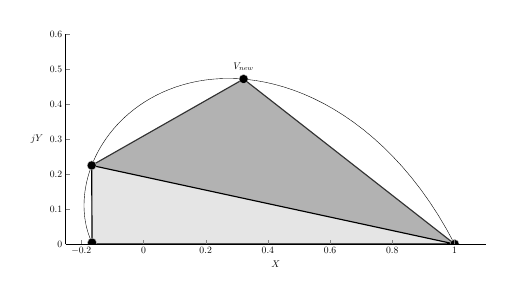
\begin{tikzpicture}[scale=0.35]

\begin{axis}[%
width=6in,
height=3in,
scale only axis,
axis on top=true,
xmin=-0.25,
xmax=1.1,
ymin=0,
ymax=0.6,
axis x line*=bottom,
axis y line*=left,
xlabel={$X$},
ylabel={$jY$},
xtick={-0.2,0,0.2,0.4,0.6,0.8,1},
ylabel style={rotate=-90},
ytick distance = 0.1
]
\addplot [color=black, forget plot]
  table[row sep=crcr]{%
1	0\\
0.97439570184454	0.0422189617067992\\
0.947664543045514	0.0822759496468887\\
0.919926652366486	0.120178744754836\\
0.891298754255365	0.155940000451509\\
0.8618940502982	0.189576974160811\\
0.831822115043362	0.221111260695846\\
0.801188805749226	0.250568528073344\\
0.770096185596349	0.277978256282022\\
0.738642459894664	0.303373479497687\\
0.706921924807467	0.326790532205477\\
0.675024928106738	0.34826879965765\\
0.643037841468705	0.367850473063845\\
0.611043043814387	0.385580309879881\\
0.579118915197029	0.401505399530848\\
0.547339840736992	0.415674934874619\\
0.515776224104452	0.428139989683019\\
0.484494510051408	0.438953302389642\\
0.453557215496707	0.448169066325949\\
0.423022968671182	0.455842726640583\\
0.392946555834355	0.462030784071105\\
0.363378975079551	0.466790605712337\\
0.334367496750526	0.47018024290145\\
0.305955729999881	0.472258256316704\\
0.278183695027438	0.473083548364434\\
0.251087900545453	0.472715202907487\\
0.224701426026886	0.471212332367794\\
0.199054008302929	0.468633932216212\\
0.174172132086558	0.465038742844109\\
0.150079124009928	0.460485118793442\\
0.126795249774977	0.455030905305267\\
0.104337814028549	0.448733322130736\\
0.0827212625856707	0.441648854533653\\
0.0619572866372231	0.433833151399599\\
0.0420549285911807	0.425340930353435\\
0.0230206892096995	0.416225889774718\\
0.00485863571765297	0.406540627589113\\
-0.0124294894283334	0.396336566703324\\
-0.0288441594077422	0.385663886941331\\
-0.0443879538246941	0.374571463330791\\
-0.0590654496872783	0.363106810580375\\
-0.0728831128341696	0.351316033581455\\
-0.0858491900514256	0.339243783761024\\
-0.0979736021088205	0.326933221106879\\
-0.109267837931654	0.314425981681024\\
-0.119744850110663	0.301762150432819\\
-0.129418951939533	0.288980239119696\\
-0.138305716156523	0.27611716914017\\
-0.146421875553965	0.263208259081419\\
-0.153785225606871	0.250287216781869\\
-0.160414529259544	0.237386135707918\\
-0.166329423997092	0.224535495443257\\
-0.171550331316981	0.211764166088996\\
-0.176098368704256	0.199099416373151\\
-0.179995264202967	0.1865669252688\\
-0.183263273665422	0.17419079692148\\
-0.185925100750451	0.161993578688022\\
-0.18800381973163	0.149996282091108\\
-0.189522801166623	0.138218406496255\\
-0.190505640469335	0.126677965320733\\
-0.190976089417432	0.11539151458703\\
-0.190957990619064	0.104374183636905\\
-0.190475214954231	0.0936397078257794\\
-0.18955160199825	0.083200463021171\\
-0.18821090342712	0.073067501733078\\
-0.186476729397344	0.0632505907086381\\
-0.18437249788586	0.0537582498279896\\
-0.181921386969236	0.0445977921430479\\
-0.179146290015116	0.0357753649058401\\
-0.176069773753131	0.0272959914381072\\
-0.172714039187066	0.0191636136990689\\
-0.169100885305011	0.0113811354135165\\
-0.16 0\\
};

\draw [color=Black!80, fill=Black!30, very thick] (-0.16, 0.00) -- (-0.166329423997092, 0.224535495443257) -- (0.3218, 0.4713) -- (1,0) -- (-0.165251675539513, 0.00395046562776303);

\draw [color=Black, fill=Gray!20, very thick] (-0.165251675539513, 0.00395046562776303) -- (-0.166329423997092, 0.224535495443257) -- (1,0) -- (-0.16, 0);

\node [circle, draw, Black!20, fill=Black!80, fill=Black, minimum size=1pt] at (-0.165251675539513, 0.00395046562776303) {};
\node [circle, draw, Black!20, fill=Black!80, fill=Black, minimum size=1pt] at (-0.166329423997092, 0.224535495443257) {};
\node [circle, draw, Black!20, fill=Black!80, fill=Black, minimum size=1pt] at (1,0) {};
\node [circle, draw, Black!20, fill=Black!80, fill=Black, minimum size=1pt, label=above:$V_{new}$] at (0.3218, 0.4713) {};

\end{axis}
\end{tikzpicture}%
\caption{}
\label{subfig:AproximacaoPoligonalZeta2}
\end{subfigure}
\\
\begin{subfigure}[t]{0.4\columnwidth}
% This file was created by matlab2tikz.
%
%The latest updates can be retrieved from
%  http://www.mathworks.com/matlabcentral/fileexchange/22022-matlab2tikz-matlab2tikz
%where you can also make suggestions and rate matlab2tikz.
%
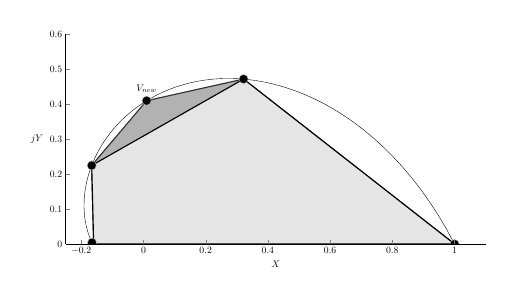
\begin{tikzpicture}[scale=0.35]

\begin{axis}[%
width=6in,
height=3in,
scale only axis,
axis on top=true,
xmin=-0.25,
xmax=1.1,
ymin=0,
ymax=0.6,
axis x line*=bottom,
axis y line*=left,
xlabel={$X$},
ylabel={$jY$},
xtick={-0.2,0,0.2,0.4,0.6,0.8,1},
ylabel style={rotate=-90},
ytick distance = 0.1
]
\addplot [color=black, forget plot]
  table[row sep=crcr]{%
1	0\\
0.97439570184454	0.0422189617067992\\
0.947664543045514	0.0822759496468887\\
0.919926652366486	0.120178744754836\\
0.891298754255365	0.155940000451509\\
0.8618940502982	0.189576974160811\\
0.831822115043362	0.221111260695846\\
0.801188805749226	0.250568528073344\\
0.770096185596349	0.277978256282022\\
0.738642459894664	0.303373479497687\\
0.706921924807467	0.326790532205477\\
0.675024928106738	0.34826879965765\\
0.643037841468705	0.367850473063845\\
0.611043043814387	0.385580309879881\\
0.579118915197029	0.401505399530848\\
0.547339840736992	0.415674934874619\\
0.515776224104452	0.428139989683019\\
0.484494510051408	0.438953302389642\\
0.453557215496707	0.448169066325949\\
0.423022968671182	0.455842726640583\\
0.392946555834355	0.462030784071105\\
0.363378975079551	0.466790605712337\\
0.334367496750526	0.47018024290145\\
0.305955729999881	0.472258256316704\\
0.278183695027438	0.473083548364434\\
0.251087900545453	0.472715202907487\\
0.224701426026886	0.471212332367794\\
0.199054008302929	0.468633932216212\\
0.174172132086558	0.465038742844109\\
0.150079124009928	0.460485118793442\\
0.126795249774977	0.455030905305267\\
0.104337814028549	0.448733322130736\\
0.0827212625856707	0.441648854533653\\
0.0619572866372231	0.433833151399599\\
0.0420549285911807	0.425340930353435\\
0.0230206892096995	0.416225889774718\\
0.00485863571765297	0.406540627589113\\
-0.0124294894283334	0.396336566703324\\
-0.0288441594077422	0.385663886941331\\
-0.0443879538246941	0.374571463330791\\
-0.0590654496872783	0.363106810580375\\
-0.0728831128341696	0.351316033581455\\
-0.0858491900514256	0.339243783761024\\
-0.0979736021088205	0.326933221106879\\
-0.109267837931654	0.314425981681024\\
-0.119744850110663	0.301762150432819\\
-0.129418951939533	0.288980239119696\\
-0.138305716156523	0.27611716914017\\
-0.146421875553965	0.263208259081419\\
-0.153785225606871	0.250287216781869\\
-0.160414529259544	0.237386135707918\\
-0.166329423997092	0.224535495443257\\
-0.171550331316981	0.211764166088996\\
-0.176098368704256	0.199099416373151\\
-0.179995264202967	0.1865669252688\\
-0.183263273665422	0.17419079692148\\
-0.185925100750451	0.161993578688022\\
-0.18800381973163	0.149996282091108\\
-0.189522801166623	0.138218406496255\\
-0.190505640469335	0.126677965320733\\
-0.190976089417432	0.11539151458703\\
-0.190957990619064	0.104374183636905\\
-0.190475214954231	0.0936397078257794\\
-0.18955160199825	0.083200463021171\\
-0.18821090342712	0.073067501733078\\
-0.186476729397344	0.0632505907086381\\
-0.18437249788586	0.0537582498279896\\
-0.181921386969236	0.0445977921430479\\
-0.179146290015116	0.0357753649058401\\
-0.176069773753131	0.0272959914381072\\
-0.172714039187066	0.0191636136990689\\
-0.169100885305011	0.0113811354135165\\
-0.16	0.0\\
};

\draw [color=Black!80, fill=Black!30, very thick] (-0.16, 0) -- (-0.166329423997092, 0.224535495443257) -- (0.0102, 0.4095) --(0.3218, 0.4713) -- (1,0) -- (-0.16, 0);

\draw [color=Black, fill=Gray!20, very thick] (-0.16, 0) -- (-0.166329423997092, 0.224535495443257) -- (0.3218, 0.4713) -- (1,0) -- (-0.16, 0);

\node [circle, draw, Black!20, fill=Black!80, fill=Black, minimum size=1pt] at (-0.165251675539513, 0.00395046562776303) {};
\node [circle, draw, Black!20, fill=Black!80, fill=Black, minimum size=1pt] at (-0.166329423997092, 0.224535495443257) {};
\node [circle, draw, Black!20, fill=Black!80, fill=Black, minimum size=1pt] at (1,0) {};
\node [circle, draw, Black!20, fill=Black!80, fill=Black, minimum size=1pt] at (0.3218, 0.4713) {};
\node [circle, draw, Black!20, fill=Black!80, fill=Black, minimum size=1pt, label=above:$V_{new}$] at (0.0102, 0.4095) {};
\end{axis}
\end{tikzpicture}%
\caption{}
\label{subfig:AproximacaoPoligonalZeta3}
\end{subfigure}
\begin{subfigure}[t]{0.4\columnwidth}
% This file was created by matlab2tikz.
%
%The latest updates can be retrieved from
%  http://www.mathworks.com/matlabcentral/fileexchange/22022-matlab2tikz-matlab2tikz
%where you can also make suggestions and rate matlab2tikz.
%
\begin{tikzpicture}[scale=0.4]

\begin{axis}[%
width=6in,
height=3in,
scale only axis,
axis on top=true,
xmin=-0.25,
xmax=1.1,
ymin=0,
ymax=0.6,
axis x line*=bottom,
axis y line*=left,
xlabel={$X$},
ylabel={$jY$},
xtick={-0.2,0,0.2,0.4,0.6,0.8,1},
ylabel style={rotate=-90},
ytick distance = 0.1
]
\addplot [color=black, forget plot]
  table[row sep=crcr]{%
1	0\\
0.97439570184454	0.0422189617067992\\
0.947664543045514	0.0822759496468887\\
0.919926652366486	0.120178744754836\\
0.891298754255365	0.155940000451509\\
0.8618940502982	0.189576974160811\\
0.831822115043362	0.221111260695846\\
0.801188805749226	0.250568528073344\\
0.770096185596349	0.277978256282022\\
0.738642459894664	0.303373479497687\\
0.706921924807467	0.326790532205477\\
0.675024928106738	0.34826879965765\\
0.643037841468705	0.367850473063845\\
0.611043043814387	0.385580309879881\\
0.579118915197029	0.401505399530848\\
0.547339840736992	0.415674934874619\\
0.515776224104452	0.428139989683019\\
0.484494510051408	0.438953302389642\\
0.453557215496707	0.448169066325949\\
0.423022968671182	0.455842726640583\\
0.392946555834355	0.462030784071105\\
0.363378975079551	0.466790605712337\\
0.334367496750526	0.47018024290145\\
0.305955729999881	0.472258256316704\\
0.278183695027438	0.473083548364434\\
0.251087900545453	0.472715202907487\\
0.224701426026886	0.471212332367794\\
0.199054008302929	0.468633932216212\\
0.174172132086558	0.465038742844109\\
0.150079124009928	0.460485118793442\\
0.126795249774977	0.455030905305267\\
0.104337814028549	0.448733322130736\\
0.0827212625856707	0.441648854533653\\
0.0619572866372231	0.433833151399599\\
0.0420549285911807	0.425340930353435\\
0.0230206892096995	0.416225889774718\\
0.00485863571765297	0.406540627589113\\
-0.0124294894283334	0.396336566703324\\
-0.0288441594077422	0.385663886941331\\
-0.0443879538246941	0.374571463330791\\
-0.0590654496872783	0.363106810580375\\
-0.0728831128341696	0.351316033581455\\
-0.0858491900514256	0.339243783761024\\
-0.0979736021088205	0.326933221106879\\
-0.109267837931654	0.314425981681024\\
-0.119744850110663	0.301762150432819\\
-0.129418951939533	0.288980239119696\\
-0.138305716156523	0.27611716914017\\
-0.146421875553965	0.263208259081419\\
-0.153785225606871	0.250287216781869\\
-0.160414529259544	0.237386135707918\\
-0.166329423997092	0.224535495443257\\
-0.171550331316981	0.211764166088996\\
-0.176098368704256	0.199099416373151\\
-0.179995264202967	0.1865669252688\\
-0.183263273665422	0.17419079692148\\
-0.185925100750451	0.161993578688022\\
-0.18800381973163	0.149996282091108\\
-0.189522801166623	0.138218406496255\\
-0.190505640469335	0.126677965320733\\
-0.190976089417432	0.11539151458703\\
-0.190957990619064	0.104374183636905\\
-0.190475214954231	0.0936397078257794\\
-0.18955160199825	0.083200463021171\\
-0.18821090342712	0.073067501733078\\
-0.186476729397344	0.0632505907086381\\
-0.18437249788586	0.0537582498279896\\
-0.181921386969236	0.0445977921430479\\
-0.179146290015116	0.0357753649058401\\
-0.176069773753131	0.0272959914381072\\
-0.172714039187066	0.0191636136990689\\
-0.169100885305011	0.0113811354135165\\
-0.16	0\\
};

%\draw [color=Black!80, fill=Black!30, very thick] (-0.16, 0) -- (-0.166329423997092, 0.224535495443257) -- (0.3218, 0.4713) -- (0.6404, 0.3694) -- (1,0) -- (-0.16, 0);

%\draw [color=Black, fill=Gray!20, very thick] (-0.165251675539513, 0.00395046562776303) -- (-0.166329423997092, 0.224535495443257) -- (0.0102, 0.4095) -- (0.3218, 0.4713) -- (1,0) -- (-0.16, 0);

\draw [color=black!70, fill=Gray!40, very thick] (-0.16, 0) -- (-0.166329423997092, 0.224535495443257) -- (0.3218, 0.4713) -- (0.6404, 0.3694) -- (1,0) -- (-0.16, 0);

\draw [color=blue, fill=matlabb!70, very thick] (-0.165251675539513, 0.00395046562776303) -- (-0.166329423997092, 0.224535495443257) -- (0.0102, 0.4095) -- (0.3218, 0.4713) -- (1,0) -- (-0.16, 0);

\node [circle, draw, Black!20, fill=Black!80, fill=Black, minimum size=1pt] at (-0.165251675539513, 0.00395046562776303) {};
\node [circle, draw, Black!20, fill=Black!80, fill=Black, minimum size=1pt] at (-0.166329423997092, 0.224535495443257) {};
\node [circle, draw, Black!20, fill=Black!80, fill=Black, minimum size=1pt] at (1,0) {};
\node [circle, draw, Black!20, fill=Black!80, fill=Black, minimum size=1pt] at (0.3218, 0.4713) {};
\node [circle, draw, Black!20, fill=Black!80, fill=Black, minimum size=1pt] at (0.0102, 0.4095) {};
\node [circle, draw, Black!20, fill=Black!80, fill=Black, minimum size=1pt, label=above:$V_{new}$] at (0.6404, 0.3694) {};

\end{axis}
\end{tikzpicture}%
\caption{}
\label{subfig:AproximacaoPoligonalZeta4}
\end{subfigure}
\caption{As primeiras quatro aproximações poligonais da curva $\zeta$-constante.}
\label{fig:AproximacoesPoligonalZeta}
\end{figure}

Para tal, utiliza-se a função $\realwn$ criada em MATLAB$\copyright$\cite{MATLAB} (código \ref{lst:RealWn} presente no anexo) para encontrar uma solução aproximada. Com tal ponto calculado e a não convexidade da cúspide tratada, é possível utilizar o algoritmo \ref{alg:AproximacaoPoligonalZeta}. Os vértices iniciais $L$ e $N$ do ramo são guardados em um vetor de vértices. Em paralelo a isso, os valores de $\omega_n$ que geram tais pontos também são armazenados. A cada iteração, o algoritmo calcula o ponto médio entre dois vértices consecutivos em cada vetor, já que a realização do primeiro depende do segundo.

Contudo, antes do algoritmo voltar para o início dos vetores, é preciso percorrer todos os pontos do vetor da iteração anterior\footnote{Como os vetores são atualizados com os novos elementos, o tamanho daqueles aumenta ($(n-1)$ pontos são adicionados a cada varredura, sendo $n$ a quantidade de pontos do vetor) durante a iteração. Assim, a execução da iteração atual termina antes de atingir o final do vetor.}. Para isso, cópias dos vetores de vértices e de pontos são inicializados, a fim de controlarem tal fluxo. Assim, quando o algoritmo terminar de percorrer o ``vetor anterior", tal conjunto é atualizado com os novos pontos e vértices calculados ao final deste processo.

Em relação ao cálculo dos pontos intermediários, a inclinação da reta que passa pelos pontos extremos locais pode ser positiva ou negativa. O uso da função $\loc$ se torna essencial, pois caso o ponto resultante for menor que zero, a reta que passa pelos pontos possui inclinação positiva, e negativa caso contrário\cite{WISNIEWSKI2019}. Assim, os setores cônicos gerados seguem a orientação desta, com centro naquele ponto calculado. A figura \ref{fig:AproximacoesPoligonalZeta} mostra as quatro primeiras iterações do algoritmo \ref{alg:AproximacaoPoligonalZeta}. É possível observar o sentido horário do fluxo para o cálculo dos vértices intermediários. Também é notável a rápida abrangência da região $\zeta$-constante.

\begin{figure}[!ht]
\centering
\begin{subfigure}[t]{0.4\columnwidth}
% This file was created by matlab2tikz.
%
%The latest updates can be retrieved from
%  http://www.mathworks.com/matlabcentral/fileexchange/22022-matlab2tikz-matlab2tikz
%where you can also make suggestions and rate matlab2tikz.
%
\begin{tikzpicture}

\begin{axis}[%
	font=\tiny,
	width=0.60037523452\textheight,
	height=0.8\textheight,
  scale only axis,
  axis on top=true,
  xmin=0.3,
  xmax=1.1,
  ymin=0,
  ymax=0.9,
  axis x line*=bottom,
  axis y line*=left,
  xlabel={$X$},
  ylabel={$jY$},
  xtick={0.4,0.5,0.6,0.7,0.8,0.9,1,1.1},
  xtick style={draw=black},
  ytick style={draw=black},
  ylabel style={rotate=-90},
  ytick distance = 0.1
  ]
  \addplot [color=black, forget plot]
    table[row sep=crcr]{%
  0.54030230586814	0.841470984807897\\
  0.534967863382191	0.833071460593297\\
  0.529768571049302	0.82470279512119\\
  0.524701459880193	0.816365672712812\\
  0.519763623176388	0.808060717031331\\
  0.514952215250233	0.799788493318601\\
  0.510264450170919	0.791549510522827\\
  0.505697600535993	0.78334422332136\\
  0.501248996267831	0.775173034042531\\
  0.49691602343458	0.767036294490186\\
  0.492696123095076	0.758934307674296\\
  0.488586790167236	0.750867329450786\\
  0.484585572319477	0.742835570073457\\
  0.480690068884672	0.734839195660667\\
  0.476897929796208	0.726878329579179\\
  0.473206854545681	0.718953053747392\\
  0.46961459116181	0.71106340985992\\
  0.466118935210123	0.703209400535282\\
  0.462717728813013	0.695390990388255\\
  0.459408859689731	0.687608107028223\\
  0.456190260215944	0.679860641984627\\
  0.453059906502422	0.672148451560422\\
  0.450015817492511	0.664471357614223\\
  0.447056054077976	0.65682914827157\\
  0.444178718232864	0.649221578565555\\
  0.441381952165015	0.641648371006764\\
  0.438663937484865	0.634109216082268\\
  0.436022894391196	0.626603772683115\\
  0.433457080873477	0.619131668459512\\
  0.430964791930477	0.611692500102562\\
  0.428544358804814	0.604285833551141\\
  0.42619414823311	0.596911204122128\\
  0.42391256171145	0.589568116561847\\
  0.421698034775829	0.582256045016197\\
  0.419549036297272	0.574974432916473\\
  0.41746406779136	0.567722692777469\\
  0.415441662741833	0.560500205903863\\
  0.413480385938019	0.553306322000374\\
  0.411578832825784	0.546140358680509\\
  0.409735628871742	0.539001600868033\\
  0.407949428940455	0.531889300084499\\
  0.40621891668436	0.524802673615316\\
  0.404542803946157	0.517740903545838\\
  0.40291983017342	0.510703135657861\\
  0.401348761845173	0.503688478175676\\
  0.399828391910187	0.496696000349422\\
  0.398357539236775	0.489724730861874\\
  0.396935048073831	0.482773656043023\\
  0.395559787522899	0.475841717874705\\
  0.394230651021055	0.468927811765217\\
  0.392946555834355	0.462030784071105\\
  0.391706442561671	0.455149429340254\\
  0.390509274648673	0.448282487246767\\
  0.389354037911772	0.44142863918402\\
  0.388239740071813	0.434586504477429\\
  0.387165410297317	0.427754636172876\\
  0.386130098757092	0.420931516350199\\
  0.385132876182003	0.414115550903467\\
  0.384172833435737	0.407305063720748\\
  0.383249081094361	0.400498290185438\\
  0.382360749034503	0.393693369908582\\
  0.381506986029992	0.386888338586634\\
  0.380686959356758	0.380081118861167\\
  0.379899854405851	0.373269510035555\\
  0.379144874304403	0.366451176477703\\
  0.378421239544366	0.359623634506574\\
  0.377728187618882	0.352784237522037\\
  0.377064972666117	0.345930159090858\\
  0.376430865120411	0.339058373644207\\
  0.375825151370604	0.332165634370895\\
  0.37524713342538	0.325248447802048\\
  0.374696128585488	0.318303044471906\\
  0.374171469122712	0.311325344899309\\
  0.373672501965436	0.3043109199563\\
  0.373198588390686	0.297254944461841\\
  0.3727491037225	0.290152142543361\\
  0.372323437036515	0.28299672292366\\
  0.371920990870632	0.275782301783101\\
  0.37154118094164	0.268501810171284\\
  0.371183435867678	0.261147382032347\\
  0.370847196896416	0.253710217667177\\
  0.370531917638833	0.246180415741187\\
  0.370237063808491	0.238546764541796\\
  0.36996211296618	0.230796479763275\\
  0.369706554269828	0.222914871126492\\
  0.369469888229576	0.214884912789054\\
  0.369251626467901	0.206686681385867\\
  0.369051291484697	0.19829660831813\\
  0.368868416427202	0.189686465478007\\
  0.368702544864672	0.180821958508667\\
  0.368553230567724	0.171660724860641\\
  0.368420037292221	0.162149397333074\\
  0.368302538567639	0.152219138716371\\
  0.368200317489797	0.141778547631191\\
  0.368112966517885	0.130701758359581\\
  0.368040087275681	0.118807042639501\\
  0.367981290356887	0.105814611834237\\
  0.367936195134494	0.0912518826526587\\
  0.367904429574089	0.0741940133758049\\
  0.367885630051037	0.0522436648106183\\
  0.367879441171442	0\\
  };
  \addplot [color=black!70, fill=Gray!40, very thick]
    table[row sep=crcr]{%
  1	0\\
  0.999950000416665	0.00999983333416666\\
  0.999800006666578	0.0199986666933331\\
  0.999550033748988	0.0299955002024957\\
  0.999200106660978	0.0399893341866342\\
  0.998750260394966	0.0499791692706783\\
  0.998200539935204	0.0599640064794446\\
  0.99755100025328	0.0699428473375328\\
  0.996801706302619	0.0799146939691727\\
  0.995952733011994	0.089878549198011\\
  0.995004165278026	0.0998334166468282\\
  0.993956097956697	0.109778300837175\\
  0.992808635853866	0.119712207288919\\
  0.991561893714788	0.129634142619695\\
  0.990215996212637	0.139543114644236\\
  0.988771077936042	0.149438132473599\\
  0.987227283375627	0.159318206614246\\
  0.985584766909561	0.169182349066996\\
  0.983843692788121	0.179029573425824\\
  0.98200423511727	0.188858894976501\\
  0.980066577841242	0.198669330795061\\
  0.978030914724148	0.2084598998461\\
  0.975897449330606	0.218229623080869\\
  0.973666395005375	0.227977523535188\\
  0.97133797485203	0.237702626427135\\
  0.968912421710645	0.247403959254523\\
  0.966389978134513	0.257080551892155\\
  0.963770896365891	0.266731436688831\\
  0.961055438310771	0.276355648564114\\
  0.958243875512697	0.285952225104836\\
  0.955336489125606	0.29552020666134\\
  0.952333569885713	0.305058636443443\\
  0.949235418082441	0.314566560616118\\
  0.946042343528387	0.324043028394868\\
  0.942754665528346	0.333487092140814\\
  0.939372712847379	0.342897807455451\\
  0.935896823677935	0.35227423327509\\
  0.932327345606034	0.361615431964962\\
  0.92866463557651	0.370920469412983\\
  0.924909059857313	0.380188415123161\\
  0.921060994002885	0.389418342308651\\
  0.917120822816605	0.398609327984423\\
  0.913088940312308	0.40776045305957\\
  0.908965749674885	0.416870802429211\\
  0.904751663219963	0.425939465066\\
  0.900447102352677	0.43496553411123\\
  0.896052497525525	0.44394810696552\\
  0.891568288195329	0.452886285379068\\
  0.886994922779284	0.461779175541483\\
  0.882332858610121	0.470625888171158\\
  0.877582561890373	0.479425538604203\\
  0.872744507645751	0.488177246882908\\
  0.86781917967765	0.496880137843737\\
  0.862807070514761	0.505533341204847\\
  0.857708681363824	0.514135991653113\\
  0.852524522059506	0.522687228930659\\
  0.847255111013416	0.531186197920883\\
  0.841900975162269	0.539632048733969\\
  0.836462649915187	0.548023936791874\\
  0.830940679100164	0.556361022912784\\
  0.825335614909678	0.564642473395035\\
  0.819648017845479	0.572867460100481\\
  0.813878456662534	0.581035160537305\\
  0.808027508312152	0.58914475794227\\
  0.802095757884293	0.597195441362392\\
  0.796083798549056	0.605186405736039\\
  0.789992231497365	0.613116851973434\\
  0.783821665880849	0.62098598703656\\
  0.777572718750928	0.628793024018468\\
  0.771246014997107	0.636537182221968\\
  0.764842187284488	0.644217687237691\\
  0.758361875990508	0.651833771021537\\
  0.751805729140895	0.659384671971473\\
  0.74517440234487	0.666869635003698\\
  0.738468558729588	0.674287911628145\\
  0.731688868873821	0.681638760023334\\
  0.724836010740905	0.688921445110551\\
  0.717910669610943	0.696135238627357\\
  0.710913538012277	0.70327941920041\\
  0.703845315652236	0.710353272417608\\
  0.696706709347165	0.717356090899523\\
  0.689498432951747	0.724287174370143\\
  0.682221207287613	0.731145829726896\\
  0.674875760071267	0.737931371109963\\
  0.667462825841308	0.744643119970859\\
  0.659983145884982	0.751280405140293\\
  0.652437468164052	0.757842562895277\\
  0.644826547240001	0.764328937025505\\
  0.63715114419858	0.770738878898969\\
  0.629412026573697	0.777071747526824\\
  0.621609968270664	0.783326909627483\\
  0.613745749488812	0.78950373968995\\
  0.605820156643463	0.795601620036366\\
  0.597833982287298	0.801619940883777\\
  0.589788025031098	0.807558100405114\\
  0.581683089463883	0.813415504789374\\
  0.573519986072457	0.819191568300998\\
  0.565299531160354	0.82488571333845\\
  0.557022546766217	0.83049737049197\\
  0.548689860581588	0.836025978600521\\
  0.54030230586814	0.841470984807897\\
  0.367879441171442 0\\
  1 0\\
  };
  
  \node [circle, draw, Magenta, fill=black, minimum size=1pt, label=above right:$R$, scale=0.5] at (0.367879441171442, 0) {};
  \node [circle, draw, Magenta, fill=black, minimum size=1pt, label=left:$Q$, scale=0.5] at (0.54030230586814, 0.841470984807897) {};
  
  \end{axis}
  \end{tikzpicture}%
\caption{}
\label{subfig:AproximacaoPoligonalWn1}
\end{subfigure}
\begin{subfigure}[t]{0.4\columnwidth}
% This file was created by matlab2tikz.
%
%The latest updates can be retrieved from
%  http://www.mathworks.com/matlabcentral/fileexchange/22022-matlab2tikz-matlab2tikz
%where you can also make suggestions and rate matlab2tikz.
%
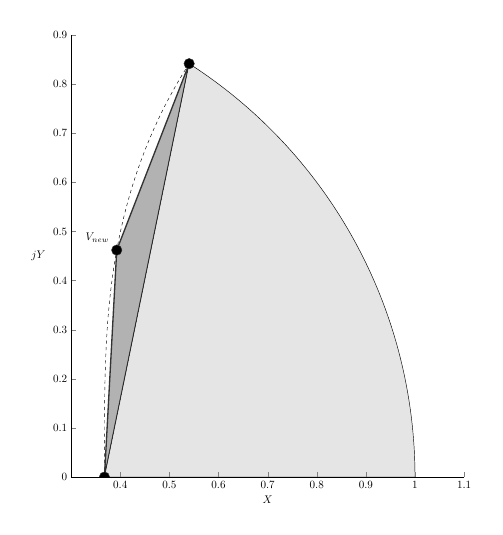
\begin{tikzpicture}[scale=0.4]

  \begin{axis}[%
  width=4.913in,
  height=5.527in,
  scale only axis,
  axis on top=true,
  xmin=0.3,
  xmax=1.1,
  ymin=0,
  ymax=0.9,
  axis x line*=bottom,
  axis y line*=left,
  xlabel={$X$},
  ylabel={$jY$},
  xtick={0.4,0.5,0.6,0.7,0.8,0.9,1,1.1},
  ylabel style={rotate=-90},
  ytick distance = 0.1
  ]
  \addplot [color=black, dashed, forget plot]
    table[row sep=crcr]{%
  0.54030230586814	0.841470984807897\\
  0.534967863382191	0.833071460593297\\
  0.529768571049302	0.82470279512119\\
  0.524701459880193	0.816365672712812\\
  0.519763623176388	0.808060717031331\\
  0.514952215250233	0.799788493318601\\
  0.510264450170919	0.791549510522827\\
  0.505697600535993	0.78334422332136\\
  0.501248996267831	0.775173034042531\\
  0.49691602343458	0.767036294490186\\
  0.492696123095076	0.758934307674296\\
  0.488586790167236	0.750867329450786\\
  0.484585572319477	0.742835570073457\\
  0.480690068884672	0.734839195660667\\
  0.476897929796208	0.726878329579179\\
  0.473206854545681	0.718953053747392\\
  0.46961459116181	0.71106340985992\\
  0.466118935210123	0.703209400535282\\
  0.462717728813013	0.695390990388255\\
  0.459408859689731	0.687608107028223\\
  0.456190260215944	0.679860641984627\\
  0.453059906502422	0.672148451560422\\
  0.450015817492511	0.664471357614223\\
  0.447056054077976	0.65682914827157\\
  0.444178718232864	0.649221578565555\\
  0.441381952165015	0.641648371006764\\
  0.438663937484865	0.634109216082268\\
  0.436022894391196	0.626603772683115\\
  0.433457080873477	0.619131668459512\\
  0.430964791930477	0.611692500102562\\
  0.428544358804814	0.604285833551141\\
  0.42619414823311	0.596911204122128\\
  0.42391256171145	0.589568116561847\\
  0.421698034775829	0.582256045016197\\
  0.419549036297272	0.574974432916473\\
  0.41746406779136	0.567722692777469\\
  0.415441662741833	0.560500205903863\\
  0.413480385938019	0.553306322000374\\
  0.411578832825784	0.546140358680509\\
  0.409735628871742	0.539001600868033\\
  0.407949428940455	0.531889300084499\\
  0.40621891668436	0.524802673615316\\
  0.404542803946157	0.517740903545838\\
  0.40291983017342	0.510703135657861\\
  0.401348761845173	0.503688478175676\\
  0.399828391910187	0.496696000349422\\
  0.398357539236775	0.489724730861874\\
  0.396935048073831	0.482773656043023\\
  0.395559787522899	0.475841717874705\\
  0.394230651021055	0.468927811765217\\
  0.392946555834355	0.462030784071105\\
  0.391706442561671	0.455149429340254\\
  0.390509274648673	0.448282487246767\\
  0.389354037911772	0.44142863918402\\
  0.388239740071813	0.434586504477429\\
  0.387165410297317	0.427754636172876\\
  0.386130098757092	0.420931516350199\\
  0.385132876182003	0.414115550903467\\
  0.384172833435737	0.407305063720748\\
  0.383249081094361	0.400498290185438\\
  0.382360749034503	0.393693369908582\\
  0.381506986029992	0.386888338586634\\
  0.380686959356758	0.380081118861167\\
  0.379899854405851	0.373269510035555\\
  0.379144874304403	0.366451176477703\\
  0.378421239544366	0.359623634506574\\
  0.377728187618882	0.352784237522037\\
  0.377064972666117	0.345930159090858\\
  0.376430865120411	0.339058373644207\\
  0.375825151370604	0.332165634370895\\
  0.37524713342538	0.325248447802048\\
  0.374696128585488	0.318303044471906\\
  0.374171469122712	0.311325344899309\\
  0.373672501965436	0.3043109199563\\
  0.373198588390686	0.297254944461841\\
  0.3727491037225	0.290152142543361\\
  0.372323437036515	0.28299672292366\\
  0.371920990870632	0.275782301783101\\
  0.37154118094164	0.268501810171284\\
  0.371183435867678	0.261147382032347\\
  0.370847196896416	0.253710217667177\\
  0.370531917638833	0.246180415741187\\
  0.370237063808491	0.238546764541796\\
  0.36996211296618	0.230796479763275\\
  0.369706554269828	0.222914871126492\\
  0.369469888229576	0.214884912789054\\
  0.369251626467901	0.206686681385867\\
  0.369051291484697	0.19829660831813\\
  0.368868416427202	0.189686465478007\\
  0.368702544864672	0.180821958508667\\
  0.368553230567724	0.171660724860641\\
  0.368420037292221	0.162149397333074\\
  0.368302538567639	0.152219138716371\\
  0.368200317489797	0.141778547631191\\
  0.368112966517885	0.130701758359581\\
  0.368040087275681	0.118807042639501\\
  0.367981290356887	0.105814611834237\\
  0.367936195134494	0.0912518826526587\\
  0.367904429574089	0.0741940133758049\\
  0.367885630051037	0.0522436648106183\\
  0.367879441171442	0\\
  };

  \draw [color=Black!80, fill=Black!30, very thick] (0.367879441171442, 0) -- (0.3929, 0.4620) -- (0.54030230586814, 0.841470984807897) -- (0.367879441171442, 0);

  \addplot [color=Black, fill=Gray!20, forget plot]
    table[row sep=crcr]{%
  1	0\\
  0.999950000416665	0.00999983333416666\\
  0.999800006666578	0.0199986666933331\\
  0.999550033748988	0.0299955002024957\\
  0.999200106660978	0.0399893341866342\\
  0.998750260394966	0.0499791692706783\\
  0.998200539935204	0.0599640064794446\\
  0.99755100025328	0.0699428473375328\\
  0.996801706302619	0.0799146939691727\\
  0.995952733011994	0.089878549198011\\
  0.995004165278026	0.0998334166468282\\
  0.993956097956697	0.109778300837175\\
  0.992808635853866	0.119712207288919\\
  0.991561893714788	0.129634142619695\\
  0.990215996212637	0.139543114644236\\
  0.988771077936042	0.149438132473599\\
  0.987227283375627	0.159318206614246\\
  0.985584766909561	0.169182349066996\\
  0.983843692788121	0.179029573425824\\
  0.98200423511727	0.188858894976501\\
  0.980066577841242	0.198669330795061\\
  0.978030914724148	0.2084598998461\\
  0.975897449330606	0.218229623080869\\
  0.973666395005375	0.227977523535188\\
  0.97133797485203	0.237702626427135\\
  0.968912421710645	0.247403959254523\\
  0.966389978134513	0.257080551892155\\
  0.963770896365891	0.266731436688831\\
  0.961055438310771	0.276355648564114\\
  0.958243875512697	0.285952225104836\\
  0.955336489125606	0.29552020666134\\
  0.952333569885713	0.305058636443443\\
  0.949235418082441	0.314566560616118\\
  0.946042343528387	0.324043028394868\\
  0.942754665528346	0.333487092140814\\
  0.939372712847379	0.342897807455451\\
  0.935896823677935	0.35227423327509\\
  0.932327345606034	0.361615431964962\\
  0.92866463557651	0.370920469412983\\
  0.924909059857313	0.380188415123161\\
  0.921060994002885	0.389418342308651\\
  0.917120822816605	0.398609327984423\\
  0.913088940312308	0.40776045305957\\
  0.908965749674885	0.416870802429211\\
  0.904751663219963	0.425939465066\\
  0.900447102352677	0.43496553411123\\
  0.896052497525525	0.44394810696552\\
  0.891568288195329	0.452886285379068\\
  0.886994922779284	0.461779175541483\\
  0.882332858610121	0.470625888171158\\
  0.877582561890373	0.479425538604203\\
  0.872744507645751	0.488177246882908\\
  0.86781917967765	0.496880137843737\\
  0.862807070514761	0.505533341204847\\
  0.857708681363824	0.514135991653113\\
  0.852524522059506	0.522687228930659\\
  0.847255111013416	0.531186197920883\\
  0.841900975162269	0.539632048733969\\
  0.836462649915187	0.548023936791874\\
  0.830940679100164	0.556361022912784\\
  0.825335614909678	0.564642473395035\\
  0.819648017845479	0.572867460100481\\
  0.813878456662534	0.581035160537305\\
  0.808027508312152	0.58914475794227\\
  0.802095757884293	0.597195441362392\\
  0.796083798549056	0.605186405736039\\
  0.789992231497365	0.613116851973434\\
  0.783821665880849	0.62098598703656\\
  0.777572718750928	0.628793024018468\\
  0.771246014997107	0.636537182221968\\
  0.764842187284488	0.644217687237691\\
  0.758361875990508	0.651833771021537\\
  0.751805729140895	0.659384671971473\\
  0.74517440234487	0.666869635003698\\
  0.738468558729588	0.674287911628145\\
  0.731688868873821	0.681638760023334\\
  0.724836010740905	0.688921445110551\\
  0.717910669610943	0.696135238627357\\
  0.710913538012277	0.70327941920041\\
  0.703845315652236	0.710353272417608\\
  0.696706709347165	0.717356090899523\\
  0.689498432951747	0.724287174370143\\
  0.682221207287613	0.731145829726896\\
  0.674875760071267	0.737931371109963\\
  0.667462825841308	0.744643119970859\\
  0.659983145884982	0.751280405140293\\
  0.652437468164052	0.757842562895277\\
  0.644826547240001	0.764328937025505\\
  0.63715114419858	0.770738878898969\\
  0.629412026573697	0.777071747526824\\
  0.621609968270664	0.783326909627483\\
  0.613745749488812	0.78950373968995\\
  0.605820156643463	0.795601620036366\\
  0.597833982287298	0.801619940883777\\
  0.589788025031098	0.807558100405114\\
  0.581683089463883	0.813415504789374\\
  0.573519986072457	0.819191568300998\\
  0.565299531160354	0.82488571333845\\
  0.557022546766217	0.83049737049197\\
  0.548689860581588	0.836025978600521\\
  0.54030230586814	0.841470984807897\\
  0.367879441171442 0\\
  1 0\\
  };

  \node [circle, draw, Black!80, fill=Black!80, fill=Black, minimum size=1pt] at (0.367879441171442, 0) {};
  \node [circle, draw, Black!80, fill=Black!80, fill=Black, minimum size=1pt] at (0.54030230586814, 0.841470984807897) {};
  \node [circle, draw, Black!80, fill=Black!80, fill=Black, minimum size=1pt, label=above left:$V_{new}$] at (0.3929, 0.4620) {};

  \end{axis}
  \end{tikzpicture}%
\caption{}
\label{subfig:AproximacaoPoligonalWn2}
\end{subfigure}
\\
\begin{subfigure}[t]{0.4\columnwidth}
% This file was created by matlab2tikz.
%
%The latest updates can be retrieved from
%  http://www.mathworks.com/matlabcentral/fileexchange/22022-matlab2tikz-matlab2tikz
%where you can also make suggestions and rate matlab2tikz.
%
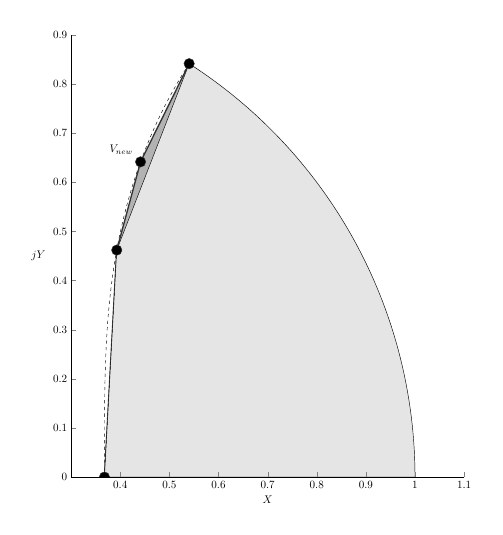
\begin{tikzpicture}[scale=0.4]

  \begin{axis}[%
  width=4.913in,
  height=5.527in,
  scale only axis,
  axis on top=true,
  xmin=0.3,
  xmax=1.1,
  ymin=0,
  ymax=0.9,
  axis x line*=bottom,
  axis y line*=left,
  xlabel={$X$},
  ylabel={$jY$},
  xtick={0.4,0.5,0.6,0.7,0.8,0.9,1,1.1},
  ylabel style={rotate=-90},
  ytick distance = 0.1
  ]
  \addplot [color=black, dashed, forget plot]
    table[row sep=crcr]{%
  0.54030230586814	0.841470984807897\\
  0.534967863382191	0.833071460593297\\
  0.529768571049302	0.82470279512119\\
  0.524701459880193	0.816365672712812\\
  0.519763623176388	0.808060717031331\\
  0.514952215250233	0.799788493318601\\
  0.510264450170919	0.791549510522827\\
  0.505697600535993	0.78334422332136\\
  0.501248996267831	0.775173034042531\\
  0.49691602343458	0.767036294490186\\
  0.492696123095076	0.758934307674296\\
  0.488586790167236	0.750867329450786\\
  0.484585572319477	0.742835570073457\\
  0.480690068884672	0.734839195660667\\
  0.476897929796208	0.726878329579179\\
  0.473206854545681	0.718953053747392\\
  0.46961459116181	0.71106340985992\\
  0.466118935210123	0.703209400535282\\
  0.462717728813013	0.695390990388255\\
  0.459408859689731	0.687608107028223\\
  0.456190260215944	0.679860641984627\\
  0.453059906502422	0.672148451560422\\
  0.450015817492511	0.664471357614223\\
  0.447056054077976	0.65682914827157\\
  0.444178718232864	0.649221578565555\\
  0.441381952165015	0.641648371006764\\
  0.438663937484865	0.634109216082268\\
  0.436022894391196	0.626603772683115\\
  0.433457080873477	0.619131668459512\\
  0.430964791930477	0.611692500102562\\
  0.428544358804814	0.604285833551141\\
  0.42619414823311	0.596911204122128\\
  0.42391256171145	0.589568116561847\\
  0.421698034775829	0.582256045016197\\
  0.419549036297272	0.574974432916473\\
  0.41746406779136	0.567722692777469\\
  0.415441662741833	0.560500205903863\\
  0.413480385938019	0.553306322000374\\
  0.411578832825784	0.546140358680509\\
  0.409735628871742	0.539001600868033\\
  0.407949428940455	0.531889300084499\\
  0.40621891668436	0.524802673615316\\
  0.404542803946157	0.517740903545838\\
  0.40291983017342	0.510703135657861\\
  0.401348761845173	0.503688478175676\\
  0.399828391910187	0.496696000349422\\
  0.398357539236775	0.489724730861874\\
  0.396935048073831	0.482773656043023\\
  0.395559787522899	0.475841717874705\\
  0.394230651021055	0.468927811765217\\
  0.392946555834355	0.462030784071105\\
  0.391706442561671	0.455149429340254\\
  0.390509274648673	0.448282487246767\\
  0.389354037911772	0.44142863918402\\
  0.388239740071813	0.434586504477429\\
  0.387165410297317	0.427754636172876\\
  0.386130098757092	0.420931516350199\\
  0.385132876182003	0.414115550903467\\
  0.384172833435737	0.407305063720748\\
  0.383249081094361	0.400498290185438\\
  0.382360749034503	0.393693369908582\\
  0.381506986029992	0.386888338586634\\
  0.380686959356758	0.380081118861167\\
  0.379899854405851	0.373269510035555\\
  0.379144874304403	0.366451176477703\\
  0.378421239544366	0.359623634506574\\
  0.377728187618882	0.352784237522037\\
  0.377064972666117	0.345930159090858\\
  0.376430865120411	0.339058373644207\\
  0.375825151370604	0.332165634370895\\
  0.37524713342538	0.325248447802048\\
  0.374696128585488	0.318303044471906\\
  0.374171469122712	0.311325344899309\\
  0.373672501965436	0.3043109199563\\
  0.373198588390686	0.297254944461841\\
  0.3727491037225	0.290152142543361\\
  0.372323437036515	0.28299672292366\\
  0.371920990870632	0.275782301783101\\
  0.37154118094164	0.268501810171284\\
  0.371183435867678	0.261147382032347\\
  0.370847196896416	0.253710217667177\\
  0.370531917638833	0.246180415741187\\
  0.370237063808491	0.238546764541796\\
  0.36996211296618	0.230796479763275\\
  0.369706554269828	0.222914871126492\\
  0.369469888229576	0.214884912789054\\
  0.369251626467901	0.206686681385867\\
  0.369051291484697	0.19829660831813\\
  0.368868416427202	0.189686465478007\\
  0.368702544864672	0.180821958508667\\
  0.368553230567724	0.171660724860641\\
  0.368420037292221	0.162149397333074\\
  0.368302538567639	0.152219138716371\\
  0.368200317489797	0.141778547631191\\
  0.368112966517885	0.130701758359581\\
  0.368040087275681	0.118807042639501\\
  0.367981290356887	0.105814611834237\\
  0.367936195134494	0.0912518826526587\\
  0.367904429574089	0.0741940133758049\\
  0.367885630051037	0.0522436648106183\\
  0.367879441171442	0\\
  };

  \draw [color=Black!80, fill=Black!30, very thick] (0.367879441171442, 0) -- (0.3929, 0.4620) -- (0.4414, 0.6416) -- (0.54030230586814, 0.841470984807897) -- (0.367879441171442, 0);

  \addplot [color=Black, fill=Gray!20, forget plot]
    table[row sep=crcr]{%
  1	0\\
  0.999950000416665	0.00999983333416666\\
  0.999800006666578	0.0199986666933331\\
  0.999550033748988	0.0299955002024957\\
  0.999200106660978	0.0399893341866342\\
  0.998750260394966	0.0499791692706783\\
  0.998200539935204	0.0599640064794446\\
  0.99755100025328	0.0699428473375328\\
  0.996801706302619	0.0799146939691727\\
  0.995952733011994	0.089878549198011\\
  0.995004165278026	0.0998334166468282\\
  0.993956097956697	0.109778300837175\\
  0.992808635853866	0.119712207288919\\
  0.991561893714788	0.129634142619695\\
  0.990215996212637	0.139543114644236\\
  0.988771077936042	0.149438132473599\\
  0.987227283375627	0.159318206614246\\
  0.985584766909561	0.169182349066996\\
  0.983843692788121	0.179029573425824\\
  0.98200423511727	0.188858894976501\\
  0.980066577841242	0.198669330795061\\
  0.978030914724148	0.2084598998461\\
  0.975897449330606	0.218229623080869\\
  0.973666395005375	0.227977523535188\\
  0.97133797485203	0.237702626427135\\
  0.968912421710645	0.247403959254523\\
  0.966389978134513	0.257080551892155\\
  0.963770896365891	0.266731436688831\\
  0.961055438310771	0.276355648564114\\
  0.958243875512697	0.285952225104836\\
  0.955336489125606	0.29552020666134\\
  0.952333569885713	0.305058636443443\\
  0.949235418082441	0.314566560616118\\
  0.946042343528387	0.324043028394868\\
  0.942754665528346	0.333487092140814\\
  0.939372712847379	0.342897807455451\\
  0.935896823677935	0.35227423327509\\
  0.932327345606034	0.361615431964962\\
  0.92866463557651	0.370920469412983\\
  0.924909059857313	0.380188415123161\\
  0.921060994002885	0.389418342308651\\
  0.917120822816605	0.398609327984423\\
  0.913088940312308	0.40776045305957\\
  0.908965749674885	0.416870802429211\\
  0.904751663219963	0.425939465066\\
  0.900447102352677	0.43496553411123\\
  0.896052497525525	0.44394810696552\\
  0.891568288195329	0.452886285379068\\
  0.886994922779284	0.461779175541483\\
  0.882332858610121	0.470625888171158\\
  0.877582561890373	0.479425538604203\\
  0.872744507645751	0.488177246882908\\
  0.86781917967765	0.496880137843737\\
  0.862807070514761	0.505533341204847\\
  0.857708681363824	0.514135991653113\\
  0.852524522059506	0.522687228930659\\
  0.847255111013416	0.531186197920883\\
  0.841900975162269	0.539632048733969\\
  0.836462649915187	0.548023936791874\\
  0.830940679100164	0.556361022912784\\
  0.825335614909678	0.564642473395035\\
  0.819648017845479	0.572867460100481\\
  0.813878456662534	0.581035160537305\\
  0.808027508312152	0.58914475794227\\
  0.802095757884293	0.597195441362392\\
  0.796083798549056	0.605186405736039\\
  0.789992231497365	0.613116851973434\\
  0.783821665880849	0.62098598703656\\
  0.777572718750928	0.628793024018468\\
  0.771246014997107	0.636537182221968\\
  0.764842187284488	0.644217687237691\\
  0.758361875990508	0.651833771021537\\
  0.751805729140895	0.659384671971473\\
  0.74517440234487	0.666869635003698\\
  0.738468558729588	0.674287911628145\\
  0.731688868873821	0.681638760023334\\
  0.724836010740905	0.688921445110551\\
  0.717910669610943	0.696135238627357\\
  0.710913538012277	0.70327941920041\\
  0.703845315652236	0.710353272417608\\
  0.696706709347165	0.717356090899523\\
  0.689498432951747	0.724287174370143\\
  0.682221207287613	0.731145829726896\\
  0.674875760071267	0.737931371109963\\
  0.667462825841308	0.744643119970859\\
  0.659983145884982	0.751280405140293\\
  0.652437468164052	0.757842562895277\\
  0.644826547240001	0.764328937025505\\
  0.63715114419858	0.770738878898969\\
  0.629412026573697	0.777071747526824\\
  0.621609968270664	0.783326909627483\\
  0.613745749488812	0.78950373968995\\
  0.605820156643463	0.795601620036366\\
  0.597833982287298	0.801619940883777\\
  0.589788025031098	0.807558100405114\\
  0.581683089463883	0.813415504789374\\
  0.573519986072457	0.819191568300998\\
  0.565299531160354	0.82488571333845\\
  0.557022546766217	0.83049737049197\\
  0.548689860581588	0.836025978600521\\
  0.54030230586814	0.841470984807897\\
  0.3929 0.4620\\
  0.367879441171442 0\\
  1 0\\
  };

  \node [circle, draw, Black!80, fill=Black!80, fill=Black, minimum size=1pt] at (0.367879441171442, 0) {};
  \node [circle, draw, Black!80, fill=Black!80, fill=Black, minimum size=1pt] at (0.54030230586814, 0.841470984807897) {};
  \node [circle, draw, Black!80, fill=Black!80, fill=Black, minimum size=1pt] at (0.3929, 0.4620) {};
  \node [circle, draw, Black!80, fill=Black!80, fill=Black, minimum size=1pt, label=above left:$V_{new}$] at (0.4414, 0.6416) {};

  \end{axis}
  \end{tikzpicture}%
\caption{}
\label{subfig:AproximacaoPoligonalWn3}
\end{subfigure}
\begin{subfigure}[t]{0.4\columnwidth}
% This file was created by matlab2tikz.
%
%The latest updates can be retrieved from
%  http://www.mathworks.com/matlabcentral/fileexchange/22022-matlab2tikz-matlab2tikz
%where you can also make suggestions and rate matlab2tikz.
%
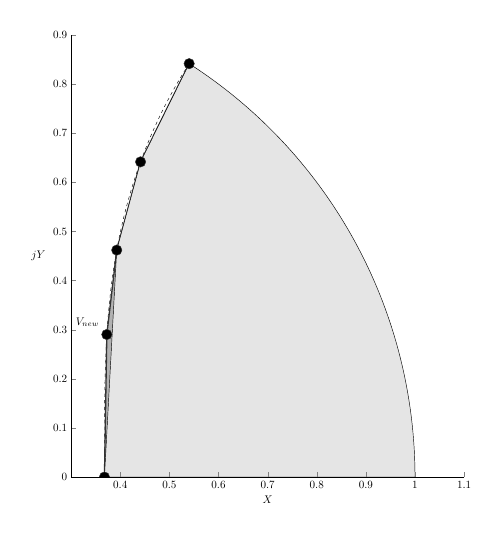
\begin{tikzpicture}[scale=0.4]

  \begin{axis}[%
  width=4.913in,
  height=5.527in,
  scale only axis,
  axis on top=true,
  xmin=0.3,
  xmax=1.1,
  ymin=0,
  ymax=0.9,
  axis x line*=bottom,
  axis y line*=left,
  xlabel={$X$},
  ylabel={$jY$},
  xtick={0.4,0.5,0.6,0.7,0.8,0.9,1,1.1},
  ylabel style={rotate=-90},
  ytick distance = 0.1
  ]
  \addplot [color=black, dashed, forget plot]
    table[row sep=crcr]{%
  0.54030230586814	0.841470984807897\\
  0.534967863382191	0.833071460593297\\
  0.529768571049302	0.82470279512119\\
  0.524701459880193	0.816365672712812\\
  0.519763623176388	0.808060717031331\\
  0.514952215250233	0.799788493318601\\
  0.510264450170919	0.791549510522827\\
  0.505697600535993	0.78334422332136\\
  0.501248996267831	0.775173034042531\\
  0.49691602343458	0.767036294490186\\
  0.492696123095076	0.758934307674296\\
  0.488586790167236	0.750867329450786\\
  0.484585572319477	0.742835570073457\\
  0.480690068884672	0.734839195660667\\
  0.476897929796208	0.726878329579179\\
  0.473206854545681	0.718953053747392\\
  0.46961459116181	0.71106340985992\\
  0.466118935210123	0.703209400535282\\
  0.462717728813013	0.695390990388255\\
  0.459408859689731	0.687608107028223\\
  0.456190260215944	0.679860641984627\\
  0.453059906502422	0.672148451560422\\
  0.450015817492511	0.664471357614223\\
  0.447056054077976	0.65682914827157\\
  0.444178718232864	0.649221578565555\\
  0.441381952165015	0.641648371006764\\
  0.438663937484865	0.634109216082268\\
  0.436022894391196	0.626603772683115\\
  0.433457080873477	0.619131668459512\\
  0.430964791930477	0.611692500102562\\
  0.428544358804814	0.604285833551141\\
  0.42619414823311	0.596911204122128\\
  0.42391256171145	0.589568116561847\\
  0.421698034775829	0.582256045016197\\
  0.419549036297272	0.574974432916473\\
  0.41746406779136	0.567722692777469\\
  0.415441662741833	0.560500205903863\\
  0.413480385938019	0.553306322000374\\
  0.411578832825784	0.546140358680509\\
  0.409735628871742	0.539001600868033\\
  0.407949428940455	0.531889300084499\\
  0.40621891668436	0.524802673615316\\
  0.404542803946157	0.517740903545838\\
  0.40291983017342	0.510703135657861\\
  0.401348761845173	0.503688478175676\\
  0.399828391910187	0.496696000349422\\
  0.398357539236775	0.489724730861874\\
  0.396935048073831	0.482773656043023\\
  0.395559787522899	0.475841717874705\\
  0.394230651021055	0.468927811765217\\
  0.392946555834355	0.462030784071105\\
  0.391706442561671	0.455149429340254\\
  0.390509274648673	0.448282487246767\\
  0.389354037911772	0.44142863918402\\
  0.388239740071813	0.434586504477429\\
  0.387165410297317	0.427754636172876\\
  0.386130098757092	0.420931516350199\\
  0.385132876182003	0.414115550903467\\
  0.384172833435737	0.407305063720748\\
  0.383249081094361	0.400498290185438\\
  0.382360749034503	0.393693369908582\\
  0.381506986029992	0.386888338586634\\
  0.380686959356758	0.380081118861167\\
  0.379899854405851	0.373269510035555\\
  0.379144874304403	0.366451176477703\\
  0.378421239544366	0.359623634506574\\
  0.377728187618882	0.352784237522037\\
  0.377064972666117	0.345930159090858\\
  0.376430865120411	0.339058373644207\\
  0.375825151370604	0.332165634370895\\
  0.37524713342538	0.325248447802048\\
  0.374696128585488	0.318303044471906\\
  0.374171469122712	0.311325344899309\\
  0.373672501965436	0.3043109199563\\
  0.373198588390686	0.297254944461841\\
  0.3727491037225	0.290152142543361\\
  0.372323437036515	0.28299672292366\\
  0.371920990870632	0.275782301783101\\
  0.37154118094164	0.268501810171284\\
  0.371183435867678	0.261147382032347\\
  0.370847196896416	0.253710217667177\\
  0.370531917638833	0.246180415741187\\
  0.370237063808491	0.238546764541796\\
  0.36996211296618	0.230796479763275\\
  0.369706554269828	0.222914871126492\\
  0.369469888229576	0.214884912789054\\
  0.369251626467901	0.206686681385867\\
  0.369051291484697	0.19829660831813\\
  0.368868416427202	0.189686465478007\\
  0.368702544864672	0.180821958508667\\
  0.368553230567724	0.171660724860641\\
  0.368420037292221	0.162149397333074\\
  0.368302538567639	0.152219138716371\\
  0.368200317489797	0.141778547631191\\
  0.368112966517885	0.130701758359581\\
  0.368040087275681	0.118807042639501\\
  0.367981290356887	0.105814611834237\\
  0.367936195134494	0.0912518826526587\\
  0.367904429574089	0.0741940133758049\\
  0.367885630051037	0.0522436648106183\\
  0.367879441171442	0\\
  };

  \draw [color=Black!80, fill=Black!30, very thick] (0.367879441171442, 0) -- (0.3727, 0.2902) -- (0.3929, 0.4620) -- (0.4414, 0.6416) -- (00.5403, 0.8415) -- (0.367879441171442, 0);

  \addplot [color=Black, fill=Gray!20, forget plot]
    table[row sep=crcr]{%
  1	0\\
  0.999950000416665	0.00999983333416666\\
  0.999800006666578	0.0199986666933331\\
  0.999550033748988	0.0299955002024957\\
  0.999200106660978	0.0399893341866342\\
  0.998750260394966	0.0499791692706783\\
  0.998200539935204	0.0599640064794446\\
  0.99755100025328	0.0699428473375328\\
  0.996801706302619	0.0799146939691727\\
  0.995952733011994	0.089878549198011\\
  0.995004165278026	0.0998334166468282\\
  0.993956097956697	0.109778300837175\\
  0.992808635853866	0.119712207288919\\
  0.991561893714788	0.129634142619695\\
  0.990215996212637	0.139543114644236\\
  0.988771077936042	0.149438132473599\\
  0.987227283375627	0.159318206614246\\
  0.985584766909561	0.169182349066996\\
  0.983843692788121	0.179029573425824\\
  0.98200423511727	0.188858894976501\\
  0.980066577841242	0.198669330795061\\
  0.978030914724148	0.2084598998461\\
  0.975897449330606	0.218229623080869\\
  0.973666395005375	0.227977523535188\\
  0.97133797485203	0.237702626427135\\
  0.968912421710645	0.247403959254523\\
  0.966389978134513	0.257080551892155\\
  0.963770896365891	0.266731436688831\\
  0.961055438310771	0.276355648564114\\
  0.958243875512697	0.285952225104836\\
  0.955336489125606	0.29552020666134\\
  0.952333569885713	0.305058636443443\\
  0.949235418082441	0.314566560616118\\
  0.946042343528387	0.324043028394868\\
  0.942754665528346	0.333487092140814\\
  0.939372712847379	0.342897807455451\\
  0.935896823677935	0.35227423327509\\
  0.932327345606034	0.361615431964962\\
  0.92866463557651	0.370920469412983\\
  0.924909059857313	0.380188415123161\\
  0.921060994002885	0.389418342308651\\
  0.917120822816605	0.398609327984423\\
  0.913088940312308	0.40776045305957\\
  0.908965749674885	0.416870802429211\\
  0.904751663219963	0.425939465066\\
  0.900447102352677	0.43496553411123\\
  0.896052497525525	0.44394810696552\\
  0.891568288195329	0.452886285379068\\
  0.886994922779284	0.461779175541483\\
  0.882332858610121	0.470625888171158\\
  0.877582561890373	0.479425538604203\\
  0.872744507645751	0.488177246882908\\
  0.86781917967765	0.496880137843737\\
  0.862807070514761	0.505533341204847\\
  0.857708681363824	0.514135991653113\\
  0.852524522059506	0.522687228930659\\
  0.847255111013416	0.531186197920883\\
  0.841900975162269	0.539632048733969\\
  0.836462649915187	0.548023936791874\\
  0.830940679100164	0.556361022912784\\
  0.825335614909678	0.564642473395035\\
  0.819648017845479	0.572867460100481\\
  0.813878456662534	0.581035160537305\\
  0.808027508312152	0.58914475794227\\
  0.802095757884293	0.597195441362392\\
  0.796083798549056	0.605186405736039\\
  0.789992231497365	0.613116851973434\\
  0.783821665880849	0.62098598703656\\
  0.777572718750928	0.628793024018468\\
  0.771246014997107	0.636537182221968\\
  0.764842187284488	0.644217687237691\\
  0.758361875990508	0.651833771021537\\
  0.751805729140895	0.659384671971473\\
  0.74517440234487	0.666869635003698\\
  0.738468558729588	0.674287911628145\\
  0.731688868873821	0.681638760023334\\
  0.724836010740905	0.688921445110551\\
  0.717910669610943	0.696135238627357\\
  0.710913538012277	0.70327941920041\\
  0.703845315652236	0.710353272417608\\
  0.696706709347165	0.717356090899523\\
  0.689498432951747	0.724287174370143\\
  0.682221207287613	0.731145829726896\\
  0.674875760071267	0.737931371109963\\
  0.667462825841308	0.744643119970859\\
  0.659983145884982	0.751280405140293\\
  0.652437468164052	0.757842562895277\\
  0.644826547240001	0.764328937025505\\
  0.63715114419858	0.770738878898969\\
  0.629412026573697	0.777071747526824\\
  0.621609968270664	0.783326909627483\\
  0.613745749488812	0.78950373968995\\
  0.605820156643463	0.795601620036366\\
  0.597833982287298	0.801619940883777\\
  0.589788025031098	0.807558100405114\\
  0.581683089463883	0.813415504789374\\
  0.573519986072457	0.819191568300998\\
  0.565299531160354	0.82488571333845\\
  0.557022546766217	0.83049737049197\\
  0.548689860581588	0.836025978600521\\
  0.54030230586814	0.841470984807897\\
  0.4414 0.6416\\
  0.3929 0.4620\\
  0.367879441171442 0\\
  1 0\\
  };

  \node [circle, draw, Black!80, fill=Black!80, fill=Black, minimum size=1pt] at (0.367879441171442, 0) {};
  \node [circle, draw, Black!80, fill=Black!80, fill=Black, minimum size=1pt] at (0.54030230586814, 0.841470984807897) {};
  \node [circle, draw, Black!80, fill=Black!80, fill=Black, minimum size=1pt] at (0.3929, 0.4620) {};
  \node [circle, draw, Black!80, fill=Black!80, fill=Black, minimum size=1pt] at (0.4414, 0.6416) {};
  \node [circle, draw, Black!80, fill=Black!80, fill=Black, minimum size=1pt, label=above left:$V_{new}$] at (0.3727, 0.2902) {};

  \end{axis}
  \end{tikzpicture}%
\caption{}
\label{subfig:AproximacaoPoligonalWn4}
\end{subfigure}
\caption{As primeiras quatro aproximações poligonais da curva $\omega_n$-constante.}
\label{fig:AproximacoesPoligonalWn}
\end{figure}

Para a região $\omega_n$-constante, a ideia é similar. A aproximação inicial utiliza-se de apenas um setor cônico voltado para a direita com centro em $R = \z(\zeta_{max},\omega_n)$. O ângulo $\theta$ em \eqref{eq:LMIESetorConicoDireito} é definido a partir do ângulo entre a reta $\overline{QR}$ e o eixo real, onde $Q = \z(\zeta_{min},\omega_n)$.

Caso esta região não seja factível, basta calcular o ponto intermediário entre $Q$ e $R$ e definir dois novos setores cônicos, a fim de aumentar a área. Novamente, para o novo ponto calculado, é utilizado a função $\loc$ para determinar o centro do setor cônico correspondente e, em seguida, usa-se $\angulo$ para determinar seu ângulo. Assim, a cada iteração, o algoritmo \ref{alg:AproximacaoPoligonalWn} adiciona dois novos setores cônicos e os intersecta com as regiões previamente definidas. Ao final da varredura, o algoritmo descarta tais regiões e começa a descrever outras restrições a partir daquelas, com novos pontos calculados. A figura \ref{fig:AproximacoesPoligonalWn} mostra as quatro primeiras iterações do algoritmo \ref{alg:AproximacaoPoligonalWn}.

Assim como ocorre com a aproximação poligonal da região $\zeta$-constante, há uma rápida cobertura da região. Com poucas iterações, a área é quase totalmente coberta. Por esse motivo, a condição de parada escolhida para ambos os algoritmos \ref{alg:AproximacaoPoligonalZeta} e \ref{alg:AproximacaoPoligonalWn} foi em relação ao incremento da área de uma iteração para outra: caso o aumento de área seja menor que $1\%$ em relação à anterior, interrompe o fluxo. Apesar de simples, a média de tempo de execução para projetos que não são possíveis foi de $10,3\,\si{\second}$.

\begin{algorithm}[!ht]
\caption{Aproximação poligonal da região $\omega_n$-constante}\label{alg:AproximacaoPoligonalWn}
\begin{algorithmic}[1]
\Require $\sigma$, $\omega_n$, $T_s$
\Ensure $K$
\State $l \gets 0$
\State $Q \gets \z(\zeta_{min},\omega_n)$
\State $R \gets \z(\zeta_{max},\omega_n)$
\State $pts3 \gets$ [$\zeta_{min}$ $\zeta_{max}$]
\State $pts4 \gets pts3$
\State $vec3 \gets$ [$R$ $Q$]
\State $vec4 \gets vec3$
\State $F \gets P \succ 0$
\State $F \gets \eqref{eq:LMIEstabilidadeRelativa}$ com $r = \exp{\left(-|\sigma|T_s\right)}$ \Comment{Taxa de amortecimento}
\State $F \gets F \cap \eqref{eq:LMIESetorConicoDireito}$, com $\alpha = R$ e $\theta = \angulo(Q,R)$ \Comment{Voltado para a direita}
\State $F \gets F \cap \eqref{eq:LMIRightBounded}$, com $\alpha = R$ \Comment{Reta vertical}
\State Verificar se o problema é factível
\While{Problema for infactível}
\If{$l < $ número de elementos em $vec3 - 1$}
\State $l \gets l + 1$
\Else
\State $l \gets 1$
\State $vec3 \gets vec4$
\State $pts1 \gets pts2$
\EndIf
\State $F \gets$ \O \Comment{Descarta as restrições anteriores}
\State $F \gets P \succ 0$
\State $F \gets \eqref{eq:LMIEstabilidadeRelativa}$ com $r = \exp{\left(-|\sigma|T_s\right)}$ \Comment{Taxa de amortecimento}
\State $pt_{new2} \gets (pts3(l)+pts3(l+1))/2$
\State $V_{new2} \gets \z(pt_{new2}, \omega_n)$
\State $pts4 \gets$ [$pts4$ $pt_{new2}$]
\State Orderna de forma decrescente $pts4$
\State $vec4 \gets$ [$vec4$ $V_{new2}$]
\State Orderna de forma decrescente $vec4$
\State $F \gets F \cap \eqref{eq:LMIRightBounded}$, com $\alpha = N$ \Comment{Reta vertical}
\For{$m = 1$ até número de elementos de $vec3-1$}
\State $u_2 \gets \loc(vec4(m),vec4(m+1))$
\State $F \gets F \cap \eqref{eq:LMIESetorConicoDireito}$, com $\alpha = u_2$ e $\theta = \angulo(vec4(m),u_2)$
\EndFor
\State Verificar se o problema é factível
\EndWhile
\State $K \gets ZP^{-1}$
\end{algorithmic}
\end{algorithm}